%%%%%%%%%%%%%%%%%%%%%%%%%%%%%%%%%%%%%%%%%%%%%%%%%%%%%%%%%%
%
% Vzor pro sazbu kvalifikační práce
%
% Západočeská univerzita v Plzni
% Fakulta aplikovaných věd
% Katedra informatiky a výpočetní techniky
%
% Petr Lobaz, lobaz@kiv.zcu.cz, 2016/03/14
%
%%%%%%%%%%%%%%%%%%%%%%%%%%%%%%%%%%%%%%%%%%%%%%%%%%%%%%%%%%

% Možné jazyky práce: czech, english
% Možné typy práce: BP (bakalářská), DP (diplomová)
\documentclass[czech,BP]{thesiskiv}

% Definujte údaje pro vstupní strany
%
% Jméno a příjmení; kvůli textu prohlášení určete, 
% zda jde o mužské, nebo ženské jméno.
\author{Jan Hinterholzinger}
\declarationmale

%alternativa: 
%\declarationfemale

% Název práce
\title{Softwarová podpora organizace předmětů TSP}

% 
% Texty abstraktů (anglicky, česky)
%
\abstracttexten{
	The bachelor thesis deals with the design of a system to support the organization of TSP subjects. The aim is to design and implement a robust web application with controlled access, which is based on the specification of the subject. Part of the work is to select a suitable framework, describe use cases and build the structure of the database model. The design of the application takes into account the requirements for modularity, responsiveness and possibilities for future expansion. During the development of the application, emphasis was placed especially on usability, reliability and security. The resulting application is thoroughly tested with prepared tests.
}

\abstracttextcz{
	Bakalářská práce se zabývá návrhem systému pro podporu organizace předmětů TSP. Cílem je navrhnout a implementovat robustní webovou aplikaci s~řízeným přístupem, která vychází ze specifikace předmětu. Součástí práce je zvolení vhodného frameworku, popsání případů užití a sestavení struktury modelu databáze. Návrh aplikace zohledňuje požadavky na modularitu, responzivitu a možnosti budoucího rozšíření. Při vývoji aplikace byl kladen důraz zejména na použitelnost, spolehlivost a bezpečnost. Výsledná aplikace je důkladně otestována připravenými testy.
}

% Na titulní stranu a do textu prohlášení se automaticky vkládá 
% aktuální rok, resp. datum. Můžete je změnit:
%\titlepageyear{2016}
%\declarationdate{1. března 2016}

% Ve zvláštních případech je možné ovlivnit i ostatní texty:
%
%\university{Západočeská univerzita v Plzni}
%\faculty{Fakulta aplikovaných věd}
%\department{Katedra informatiky a výpočetní techniky}
%\subject{Bakalářská práce}
%\titlepagetown{Plzeň}
%\declarationtown{Plzni}

%%%%%%%%%%%%%%%%%%%%%%%%%%%%%%%%%%%%%%%%%%%%%%%%%%%%%%%%%%
%
% DODATEČNÉ BALÍČKY PRO SAZBU
% Jejich užívání či neužívání záleží na libovůli autora 
% práce
%
%%%%%%%%%%%%%%%%%%%%%%%%%%%%%%%%%%%%%%%%%%%%%%%%%%%%%%%%%%

% Zařadit literaturu do obsahu
\usepackage[nottoc,notlot,notlof]{tocbibind}

% Umožňuje vkládání obrázků
\usepackage[pdftex]{graphicx}

% Odkazy v PDF jsou aktivní; navíc se automaticky vkládá
% balíček 'url', který umožňuje např. dělení slov
% uvnitř URL
\usepackage[pdftex]{hyperref}
\usepackage{pdfpages}
\hypersetup{colorlinks=true,
  unicode=true,
  linkcolor=black,
  citecolor=black,
  urlcolor=black,
  bookmarksopen=true}

% Při používání citačního stylu csplainnatkiv
% (odvozen z csplainnat, http://repo.or.cz/w/csplainnat.git)
% lze snadno modifikovat vzhled citací v textu
\usepackage[numbers,sort&compress]{natbib}

\usepackage{float}
\usepackage{dirtree}

\usepackage{blindtext}
\usepackage{multicol}

% Barvičky
\usepackage{xcolor}
\colorlet{mygray}{black!30}
\colorlet{mygreen}{green!60!blue}
\colorlet{mymauve}{red!60!blue}
% Vkládání formátovaného zdrojového kódu

\usepackage{amssymb}
\usepackage{booktabs,xltabular}
\usepackage{listings}
\renewcommand{\lstlistingname}{Ukázka kódu}
\renewcommand\lstlistlistingname{Seznam ukázek kódu}
\lstset{
	backgroundcolor=\color{gray!10},  
	basicstyle=\ttfamily,
	columns=fullflexible,
	breakatwhitespace=false,      
	breaklines=true,                
	captionpos=b,                    
	commentstyle=\color{mygreen}, 
	extendedchars=true,              
	frame=single,                   
	keepspaces=true,             
	keywordstyle=\color{blue},      
	language=php,                 
	numbers=none,                
	numbersep=5pt,
	numberbychapter=false,
	numberstyle=\tiny\color{blue}, 
	rulecolor=\color{mygray},        
	showspaces=false,               
	showtabs=false,
	showstringspaces=false,
	stepnumber=1,                  
	stringstyle=\color{mymauve},    
	tabsize=3,                      
	title=\lstname,
	numbers=left,      
	extendedchars=true,
	literate={á}{{\'a}}1 {ã}{{\~a}}1 {é}{{\'e}}1
}
\overfullrule 10pt
%%%%%%%%%%%%%%%%%%%%%%%%%%%%%%%%%%%%%%%%%%%%%%%%%%%%%%%%%%
%
% VLASTNÍ TEXT PRÁCE
%
%%%%%%%%%%%%%%%%%%%%%%%%%%%%%%%%%%%%%%%%%%%%%%%%%%%%%%%%%%
\begin{document}
%
\maketitle
%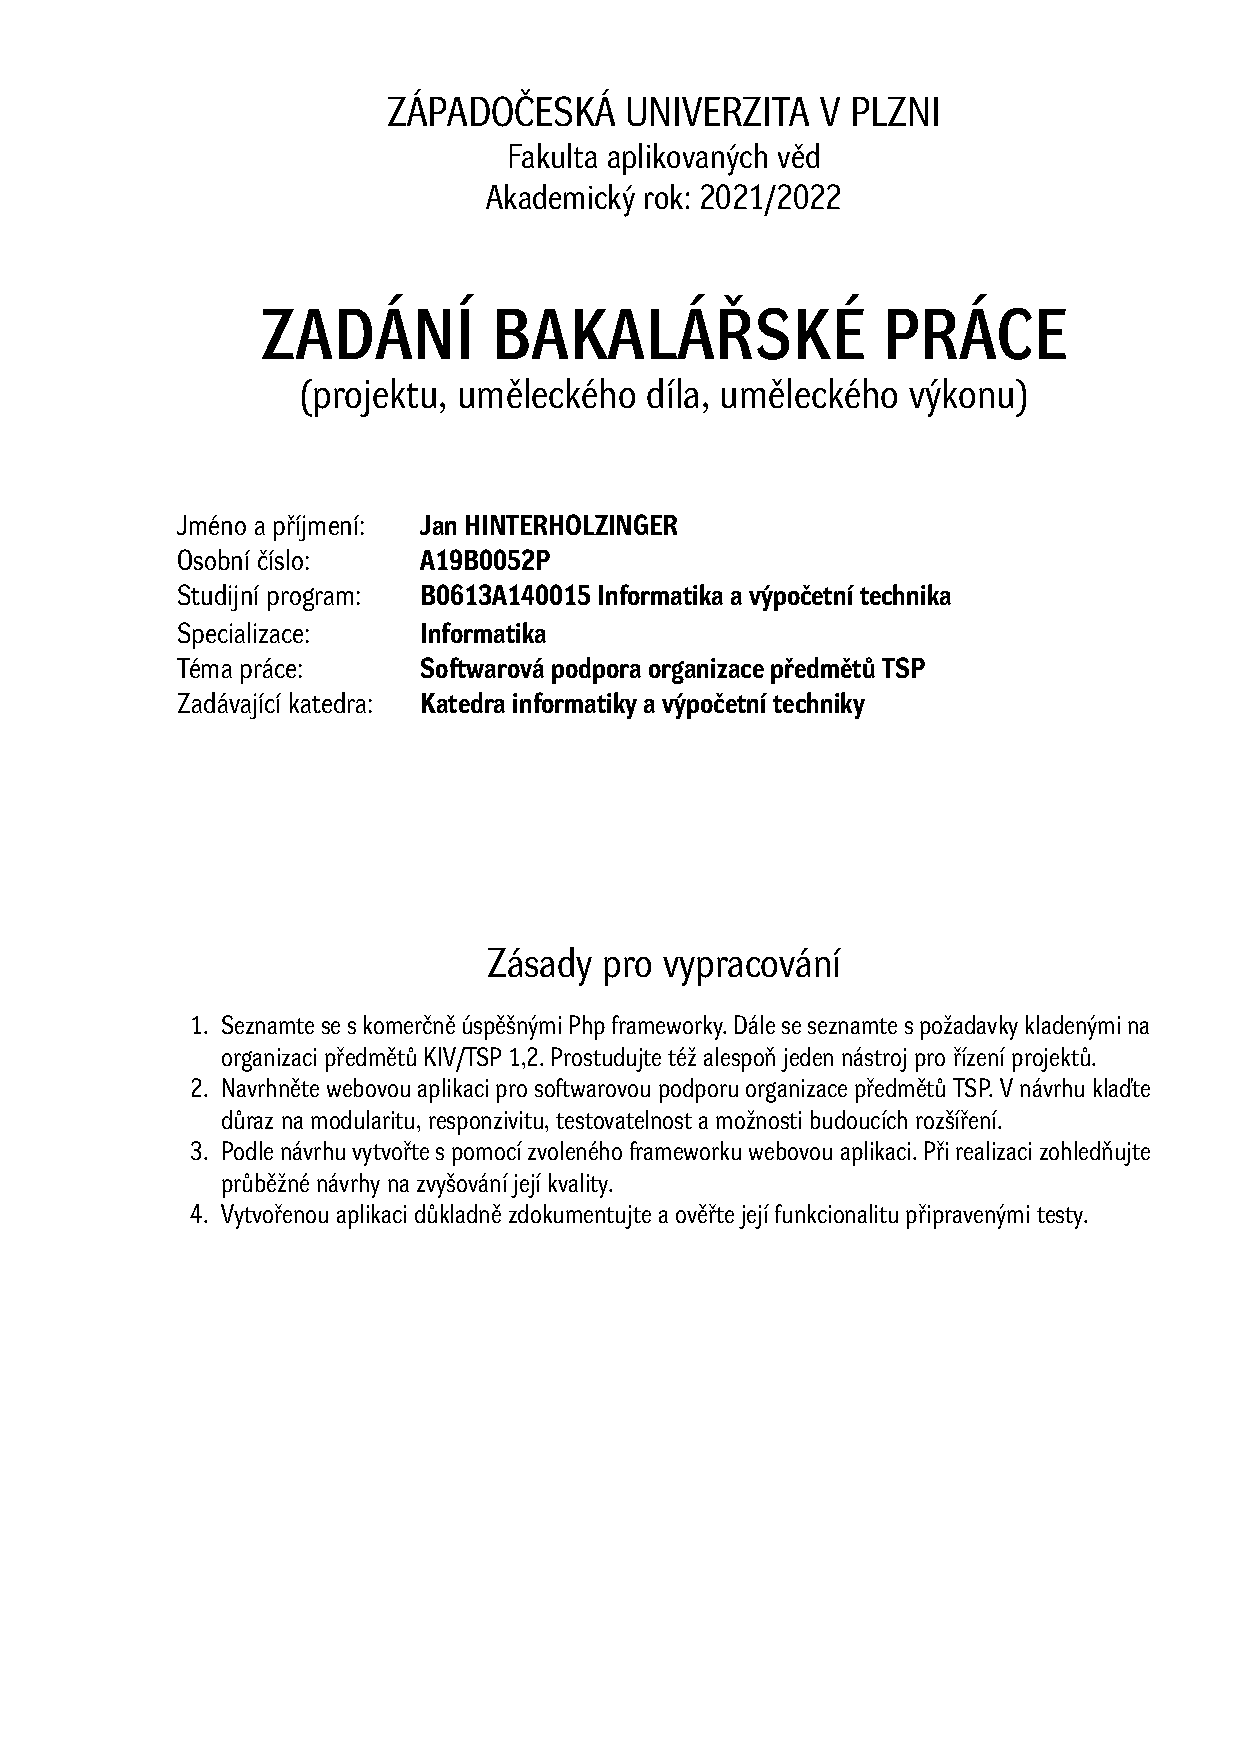
\includepdf[pages=-]{include/zadani.pdf}[H]
\tableofcontents
\chapter{Úvod}
	\par Na Katedře informatiky a výpočetní techniky vzniká nový předmět \uv{Týmový softwarový projekt} (KIV/TSP1 a KIV/TSP2) určený pro studenty navazujícího studia. Podstatou předmětu je vypracování zadaného tématu ve skupinkách studentů, kdy studenti přijdou do styku s~týmovou prací, řízením projektu a dalšími interními procesy.
	\par Na obou předmětech je doba pro řešení projektu, dva semestry rozdělené do dvou předmětů a ročníků. Budou zapojeny čtyři skupiny lidí garant, zadavatelé, mentoři a studenti, což bude klást poměrně značné nároky na organizaci předmětu. Bylo rozhodnuto o~vytvoření webové aplikace, která všem zúčastněným stranám zjednoduší zadávání témat a evidenci postupu prací projektu. Cílem aplikace je umožnit lepší informovanost a zapojení studentů, řešení evidence zadavatelů a možnosti sdílení informací mezi mentorem, garantem a vedoucími týmů.
	\par Cílem práce je vyvinout zmíněnou webovou aplikaci dle specifikace předmětu a požadavků jeho garanta. Předpokládá se, že aplikace bude v~budoucnu nadále rozšiřována. Je proto žádoucí, aby aplikace byla dostatečně robustní, modulární a důkladně otestována.
	\par Pro tak značný rozsah časový i personální by již pravděpodobně nestačila evidence pomocí spreadsheet\footnote{tabulkový procesor} tabulky, byť potenciálně sdílené.
\chapter{Specifikace požadavků}
\par Specifikace požadavků se řídí průběhem a organizací předmětů TSP. V~době vývoje aplikace se díky aktivní přípravě těchto předmětů několikrát požadavky změnily a tedy muselo být počítáno s~průběžnou aktualizací specifikace. Z~tohoto důvodu je potřeba aplikaci psát s~dostatečným odstupem a přiměřeně obecně, aby odolávala drobným změnám specifikace. Aplikaci bylo stanoveno jméno PSTSP (Podpůrný software TSP).
\section{Organizace předmětů TSP}
	\par Výuka předmětů TSP je rozdělena do dvou semestrů, a tedy do dvou předmětů KIV/TSP1 vyučovaného v~letním semestru 1. ročníku a KIV/TSP2 v~zimním semestru 2. ročníku. Řešení týmového projektu tedy bude překračovat hranice ročníku a v~mnoha částech se organizace předmětů bude překrývat.
	\par Životní cyklus bude nejčastěji probíhat následovně. 
	\begin{itemize}
		\item Garant přijímá od domluvených zadavatelů jejich zadání, která mají studentské týmy řešit. Tato zadání společně s~PDF souborem vloží do PSTSP pro zvolené období předmětu.
		\item Před začátkem TSP budoucí vedoucí týmu zažádá garanta o~založení účtu v~PSTSP s~rolí \uv{Vedoucí}. Vedoucí týmu společně s~dalšími studenty sestaví tým a vloží informace o~týmu.
		\item Sbor mentorů vyhodnotí zadání z~hledisek náročnosti, vhodnosti, technologické proveditelnosti a případně požádá zadavatele o~jejich korekci či upřesnění. Z~opravených zadání se stanou témata.
		\item Poté co jsou témata projektů zveřejněna, vedoucí týmu (na základě rozhodnutí v~týmu) projeví zájem o~jedno či více zvolených témat.
		\item Mentor zodpovědný za téma ohodnotí vhodnost zvoleného tématu pro daný tým na základě zájmu a deklarovaných schopností týmu.
		\item Garant následně podle rozhodnutí mentora a zájmu týmu definitivně přiřadí některé z~témat týmu. Přiřazením tématu vzniká projekt.
		\item Tým řeší projekt a postup řešení vkládá do PSTSP.
		\item Mentor na základě postupu řešení týmu kontroluje a potvrzuje postup týmu.
		\item Na závěru předmětu TSP se koná obhajoba projektu, jejíž výsledek se zapíše do PSTSP.
	\end{itemize}
\section{Role v~PSTSP}
	\subsection{Nepřihlášený uživatel}
		\par Nepřihlášený uživatel je každý návštěvník aplikace, který se neprokáže svými přihlašovacími údaji. Takový uživatel může ve skutečnosti být student předmětu TSP, proto je mu umožněno zobrazovat vypsaná témata a již existující týmy, které hledají nové členy.
	\subsection{Vedoucí týmu}
		\par Student předmětů TSP, který zažádal garanta o~vytvoření konta. Tento uživatel je pověřen tvorbou týmu. Je mu umožněno vyjadřovat zájmy o~volná témata, které následně ohodnocuje mentor a na základě zájmu je garantem téma přiděleno. Také má povinnost evidovat v~projektu splnění kritérií, postupu a využitých zkušeností.
	\subsection{Mentor}
		\par Vyučující předmětů TSP, který má v~softwarové podpoře založený účet. Jeho úkolem je evidovat postup a kontrolovat výstupy z~týmu. Mentorovi dále bude umožněno převzít si téma, které bude mentorovat a určovat vhodnost tématu dle projevených zájmů týmů o~konkrétní téma, které mentoruje.
	\subsection{Garant}
		\par Garant je osoba, která koordinuje činnost všech ostatních skupin uživatelů. Mezi jeho hlavní náplň patří také přidávání nových témat, správa uživatelů a dalších nastavení.

\chapter{Dostupné technologie}
\section{PHP}
\par PHP je jedním z~nejoblíbenějších jazyků zpracovávaných na straně serveru v~oblasti webového vývoje. Jedná se volně dostupný skriptovací jazyk, který je spravován a vyvíjen skupinou vývojářů s~názvem The PHP Group.
\par Jazyk PHP se většinou používá na straně serveru (backend). Po jeho zpracování jsou výsledky typicky poskytovány webovým serverem. Takový server musí mít nainstalovaný modul PHP. Poté lze vkládat kód jazyka do značkovaného kódu jazyka HTML. Soubory s~PHP kódem mají koncovku .php. Jazyk je možné provozovat na velké škále operačních systémů na všech platformách.
\par Díky své jednoduchosti bývá PHP častá volba pro vývoj webových aplikací. Poskytuje dostatečné množství funkcí, aby programátor nepotřeboval přecházet na jiný jazyk a vystačil si čistě s~jazykem PHP. Jazyk je konkurentem pro jazyky jako ASP.NET, Java a Node.js, které se také zabývají webovým vývojem.
\par Díky velké popularitě jazyka vznikla velká komunita vývojářů, kteří převážně zdarma nabízejí pomoc na různých fórech \cite{PHPOkamzite}.
\section{Srovnání PHP Frameworků}
	\par Existuje několik cest jak webovou aplikaci vyvíjet. V~základu se jedná o~dva směry. Vyvíjení aplikace z~již vytvořených komponent a tvorba od úplného počátku. Oba směry mají své výhody a nevýhody. Pro rozsáhlé systémy se však posledních několik let rozmáhá použití frameworků.
	\subsection{PHP Framework}
	\par PHP framework je platforma pro tvorbu webových aplikací. Obsahuje již vytvořené knihovny pro často používané činnosti. Tvoří tak základ, na kterém mohou vývojáři stavět svůj produkt. Tento přístup je často vítaný, protože umožňuje urychlení a sjednocení vývoje.
	\par PHP framework pro vývojáře totiž řeší celou řadu problémů. Příkladem mohou být různé optimalizační nástroje, DI\footnote{Dependency Injection -- technologie vkládání závislostí} kontejner nebo komunikace s~databází. Vývojář se tak může zaměřit na vývoj samotné logiky aplikace a nezabývat se příliš repetetivními a nízkoúrovňovými záležitostmi.
	\par Bezpečnost je také jedním z~hlavních bodů, kterým se PHP Frameworky věnují. Poskytují totiž obalovací objekty nad nízkoúrovňovými funkcemi a v~nich sami vytváří bezpečností vrstvu. Pomocí frameworku prakticky bez námahy chráníte svoji aplikaci proti různým typům útokům. 
	\par Součástí frameworků bývají šablonovací sytém, který je možno při vývoji použít. Případně může vývojář zvolit jiný, který mu vyhovuje. Šablonovací enginy slouží pro prezentaci dat z~backendové části aplikace a tvoří tak HTML stránku, kterou vidí uživatel. Některé šablonovací systémy obsahují vlastní funkce například pro úpravu textu, podmíněné vykreslování nebo cykly, tj. struktury, které známe z~jiných programovacích jazyků. Zde však slouží pro zmíněnou prezentaci dat.
	\subsection{Vybrané frameworky ke srovnání}
	\par V~dnešní době již několik spousta spolehlivých frameworků, které mohou být použity. Celosvětové žebříčky popularity dlouhodobě vedou frameworky Symfony a Laravel. Oba frameworky jsou mírně rozdílné a rozhodnutí, který nasadit spočívá v~druhu použití. V~českém prostředí jim konkuruje Nette.
	\subsubsection{Laravel}
	\par Framework Laravel je možné považovat za nejrozšířenější. Mezi jeho hlavní východy patří jeho jednoduchost používání a rychlost. Pro svůj přístup k~jednoduchému použití je Laravel doporučován jako vhodný pro začátečníky ale i pro profesionály. Framework se hodí pro vytváření méně komplexních projektů.
	\par Laravel využívá šablonovací engine Blade, který je standardně dodáván společně se samotným frameworkem. Tento engine umožňuje oproti jiným rozšiřovat PHP kód, a tak provádět různé jednoduché operace pro přizpůsobení dat k~samotnému front-endu.
	\subsubsection{Symfony}
	\par Tento framework se vyznačuje zakládáním si na striktním dodržování PHP standardů a snaží se maximálně využívat různé návrhové vzory. Díky tomu jsou komponenty frameworku robustnější, což může znamenat větší časovou náročnost, na druhou stranu ale také výraznou stabilitu frameworku, a proto je vhodný pro použití na komplexnějších projektech. Další předností mohou být rozsáhlé možnosti pro vývojáře, který si může prostředí přizpůsobit svým potřebám. To však vyžaduje hlubší znalosti jazyka PHP a struktury frameworku. Pro nováčky je tedy Symfony více náročný na naučení.
	\par Jako výchozí šablonovací engine je využíván Twig, který se také řadí mezi nejpoužívanější šablonovací systémy. Oproti systému Blade obsahuje navíc další bezpečnostní vrstvu a další funkce. Twig je často využíván i samostatně, tedy bez použití back-end frameworku. To potvrzuje jeho flexibilitu.
	\subsubsection{Nette}
	\par Český projekt Nette není tolik světově známý, ale v~České republice je velice populární. Kombinuje totiž výhody obou předchozích frameworků a dosahuje velmi dobrých výsledků. Je distribuován po různých volitelných modulech. Součástí těchto modulů je i ladička\footnote{Ladící nástroj pro vylepšování aplikace} Tracy, která poskytuje rozsáhlé ladící možnosti. Svoji popularitu si nadále udržuje i díky velmi aktivní komunitě.
	\subsection{Srovnání}
	\par Jedná se o~frameworky, které jsou si velmi podobné a prostý výčet nabízených funkcí je takřka podobný. V~určitých drobnostech se však jejich použití liší.
	\subsubsection{Podobnosti}
	\par Všechny zmíněné frameworky používají při komunikaci s~databází objektově relační mapování. To znamená, že výsledky z~databáze nejsou vráceny jako pole hodnot, ale jako objekty, nad kterými lze volat další funkce. Díky tomu je možné dotazy na databázi i postupně optimalizovat a tím zrychlovat činnost aplikace.
	\par V~otázkách poskytování závislostí nabízejí všechny vlastní formu DI kontejneru.
	\par Přikládané šablonovací enginy poskytují formu dědičnosti šablon. Umožňují rozšíření vlastními funkcemi a tak upravovat výpisy.
	\subsubsection{Rozdílnosti}
	\par Světově jsou frameworky Symfony a Laravel velice oblíbené a značně zastoupené. Z~perspektivy České republiky je však Nette nejužívanější a v~tomto ohledu značně překonává i zbylé dva porovnávané frameworky.
	\par Učební křivka frameworků se liší. Zatímco Symfony se řadí mezi ty náročnější, Laravel si zakládá na své jednoduchosti a Nette tvoří pomyslný střed.
	\subsection{Výběr}
	\par Na vyvíjený projekt, který je rozsahem střední velikosti lze vhodně použít jakýkoli ze zmíněných frameworků. Výsledný výběr tak stojí na zkušenostech a osobních preferencí vývojáře.
	\par Z~důvodu toho, že vývojář i tester se již setkali s~frameworkem Nette a mají s~ním alespoň začátečnické zkušenosti, byl vybrán framework Nette.
\section{Front-end}
	\subsection{HTML a CSS}
		\par Základem webových aplikací je způsob zobrazování. Webové technologie nabízejí tvorbu elementů pomocí formátu HTML\footnote{Hyper Text Markup Language -- Značkovací jazyk pro tvorbu webových technologií} založeného na SGML\footnote{Standard Generalized Markup Language -- Obecně standardizovaný značkovací jazyk}. Vlastností tohoto formátu je tvorba webových elementů pomocí tagů, kterými se specifikují jejich vlastnosti. Dnes již naprostá většina prohlížečů zobrazuje webové stránky pomocí tohoto formátu a je prakticky synonymem pro internetové stránky \cite{HTML5aCSS3}.
		\par Další obdobně oblíbenou technologií je stylovací kaskádový jazyk CSS\footnote{Cascading Style Sheet -- technologie pro úpravu vzhledu nejen webových stránek}. Díky tomuto formátu je možné nastavovat atributy jednotlivých elementů a upravovat tak zejména jejich vzhled. Tyto styly lze aplikovat přímo do HTML tagu daného elementu nebo do blokového elementu společného pro celou stránku. Nejčastěji se však využívá importování přiloženého \texttt{.css} souboru. CSS umožňuje vzhled stránky upravovat i podle velikosti displeje zařízení a tak přizpůsobit obsah i pro menší obrazovky \cite{CSSOkamzite}.
		\par Hlavním cílem jazyka CSS je oddělovat formátovací a stylizační pravidla od obsahu stránky. Díky tomu je možné stránky snadněji udržovat a přinutit je pracovat správně v~různých webových prohlížečích, na různých platfomách, zařízení nebo dokonce při tisku \cite{HTML5aCSS3}.
	\subsection{Bootstrap}
		\par Bootstrap představuje nadstavbu nad CSS styly. Umožňuje upravovat prvky pomocí tříd a dát jim tak moderní vzhled bez potřeby upravovat styly ručně. Při správném použití tohoto frameworku je velice snadno zajištěn responzivní design webu.
	\subsection{AdminLTE}
		Ačkoli Bootstrap přichází již s~hotovou sadou stylů pro určité prvky a pro responzivitu, tak stavba celé webové aplikace by se neobešla bez četného přidávání vlastních stylů. Existují však nástavby nad technologií Bootstrap a nabízejí kompletní sadu stylů k~vytvoření informačních systémů. Jedním z~takových projektů je front-endový framework AdminLTE. 
		\par Tento framework nabízí celou řadu placených šablon, ale poskytuje i jednu velmi oblíbenou šablonu zdarma. Součástí tohoto frameworku jsou příklady použití stylů jednotlivých elementů a také předpřipravené šablony pro celé stránky.
		\par Framework využívá Bootstrap, je tedy stejně jednoduché využívat responzivitu a čerpat jeho dalších výhod. Stylování stránek tedy vypadá tak, že na hotovou HTML strukturu aplikujeme třídy již vytvořených stylů.
\section{Databáze MariaDB}
	\par Databáze je důležitá součást aplikace, která zpracovává nějaká data a je potřeba jejich uložení a rychlé přístupnosti k~nim.
	\par MariaDB databáze je relační databáze oblíbená vývojáři zejména webových projektů malé a střední velikosti. Systém MariaDB původně vznikl jako alternativní větev projektu MySQL poté co jej společnost Oracle odkoupila. MariaDB staví na své značné kompatibilitě s~databází MySQL, která je považována podle různých průzkumů za jednu z~nejoblíbenějších databází pro webové aplikace společně s~databází Oracle a MS SQL. Další přednosti systému MariaDB je její cíl zůstat open-source projektem.
	\par Díky velké kompatibilitě s~databází MySQL je možné využívat nástroje určené nativně pro MySQL i pro MariaDB. Proto pro vývoj využíváme nástroj MySQL Workbench, který pro většinu případů poskytuje stejné funkce jako pro databázi MySQL.
	\par Byla zvolena databáze MariaDB díky tomu, že se jedná o~otevřený projekt spravovaný nezávislou skupinou. Oproti tomu distribuování MySQL zdarma může být z~důvodu korporátních vlivů v~budoucnu omezeno. Je však nutno podotknout, že přechod z~MariaDB na MySQL je většinou velmi snadný a bezproblémový. Je tak možno prohlásit podporu aplikace i pro MySQL.
\section{Nástroje pro řízení projektu}
	\par Aplikace, kterou vyvíjíme, bude patřit mezi rozsahově náročnější, proto je její řešení rozděleno do dvou prací. Jedna práce (tato) se věnuje samotnému vývoji aplikace. Druhá je zaměřená na důkladné otestování aplikace, čímž má být zajištěna její kvalita a spolehlivost.
	\par Protože na aplikaci takového rozsahu pracuje více lidí, je potřeba využít takové procesy, které usnadní jednotlivé části vývoje a domluvu mezi vývojem, testováním a vedoucím práce.
\subsection{Verzovací systém}
	\par V~oblasti vývoje informačních projektů je častým nástrojem pro efektivní a produktivní vývoj verzovací systém ze skupiny Git.
	\par Tato technologie totiž umožňuje práci více vývojářů na jednom projektu současně. Jednotlivé změny v~repozitáři vývojáři seskupují do tzv. commitů. Ty v~systémech Git představují nejmenší jednotku změny v~úložišti. Commit v~sobě obsahuje informace o~upravených řádkách textových souborů a změny dalších souborů.
	\par Další důležitou funkcí Git je větvení. V~základu je v~repozitáři hlavní větev \uv{main} nebo \uv{master}, která obsahuje centrální vývoj projektu. Od této větve se oddělují další větve, dle určení. Typicky se do jednotlivých větví postupně commitují úpravy rozsáhlejší funkcionality aplikace. Díky tomu ostatní vývojáři nejsou těmito změnami zasaženi a tak si nepřekážejí.
	\par Po dokončení úprav nebo přidávání funkcionality jsou commity větve sloučeny do rodičovské větve, kde tvoří větší celek. Tato funkce se jmenuje Merge request a její starostí je přemístit commity jedné větve do jiné větve tak, aby byly změny zaneseny. Může se stát, že se změny v~obou větvích dostanou do konfliktu, poté záleží na uživateli jak konflikt vyřeší.
	\par Dostupných nadstaveb verzovacích systémů existuje celá řada. Mezi nejvýznamnější na trhu patří GitHub a GitLab.
	\par GitHub je pravděpodobně nejúspěšnější systém pro tvorbu projektů od jednotlivců nebo malých skupin. Obsahuje však výrazná omezení, která jsou sice odstraněny v~prémiovém plánu, ale v~našem případě výhody ostatních nadstaveb převažují nad výhodami GitHubu.
	\par Z~tohoto důvodu se zdá být přínosnější použít systém GitLab, který pokrývá veškeré naše požadavky. 
	\par Důležitou zmínkou je, že projekt GitLab je veden jako open-source. Díky tomu Katedra informatiky a výpočetní techniky provozuje svoji vlastní instalaci tohoto verzovacího nástroje na katedrálním serveru.
	\par To má pro studenty nesmírnou výhodu, protože během dosavadního studia již GitLab používali a mají s~ním zkušenosti. Navíc všichni zúčastnění mají na této platformě vytvořené účty, nemusí se tedy organizačně řešit vstup na novou platformu.
	\par Z~těchto důvodů jsme se v~naší volbě verzovacího systému rozhodli zvolit právě variantu GitLab s~katedrálním serverem.
\subsection{Plánování úkolů}
	\par S~rozsahem práce přichází i potřeba rozvržení práce na časové úseky a stanovení cílů. Zároveň je žádoucí, aby k~plánu měli přístup všechny zúčastněné osoby. Tyto požadavky sice splňuje množství známých nástrojů nebo sdílených úložišť. My jsme se ale rozhodli využít již námi používaný nástroj GitLab.
	\par Tento nástroj obsahuje možnosti vytváření wiki dokumentace ve formátu MarkDown, který navíc zajišťuje základní formátování.
	\par V~této dokumentační sekci máme vytvořenou jednu stránku, ve které je po týdnech rozdělena struktura naplánovaných úkolů a vzniklých dotazů.
\subsection{Issues}
	\par Různé požadavky evidujeme jako jednotlivé issues. Issues je záznam o~požadavku na aplikaci nebo úkolu, který je potřeba vykonat. Issue tak eviduje přiřazení k~člověku, který daný požadavek řeší, kompletní historii řešení požadavku, termíny pro jeho splnění, atd.
	\par Systém také poskytuje štítkování těchto issues a tím pomáhá v~jejich řazení, filtrování, seskupování i výběru. Díky štítkům můžeme totiž přiřazovat prioritu, závažnost, druh požadavku na aplikaci a jiné označení.
	\par Issues nám pomáhají ve fragmentaci  jednotlivých požadavků na aplikaci do přibližně stejně náročných dílů, které se poté ve vývoji dobře plní a je tak zajištěna přehlednost. Zároveň má tento princip i pozitivní psychologický dopad, kdy vývojáři mají dobrý pocit z~dokončeného úkolu a mají tak chuť pokračovat dalším issue.
	\par V~systému GitLab tyto issues používáme také ve funkci Board, který využívá principy kanbanu.
\subsection{Kanban}
	\par Systém Kanban je strategie řízení projektu, kdy si mezi sebou části výroby předávají výrobek. Cílem je využívat pouze ty nejnutnější zdroje.
	\par V~praxi se tento systém zobrazuje jako tabule, kde jsou rozvržené jednotlivé sloupce dle možných stavů vývoje. Následně zde máme rámečky představující výrobek, které obsahují popis jak má být produkt upraven. Podstatou věci je, že tyto rámečky následně přemisťujeme mezi jednotlivými sloupci v~závislosti na reálném stavu produktu.
	\par Obrázek \ref{fig:kanban} obsahuje snímek z~reálného použití při vývoji. Jednotlivé issues jsou rozděleny do sloupců dle jejich stavu rozpracovanosti.
	\begin{figure}[H]
		\centering
		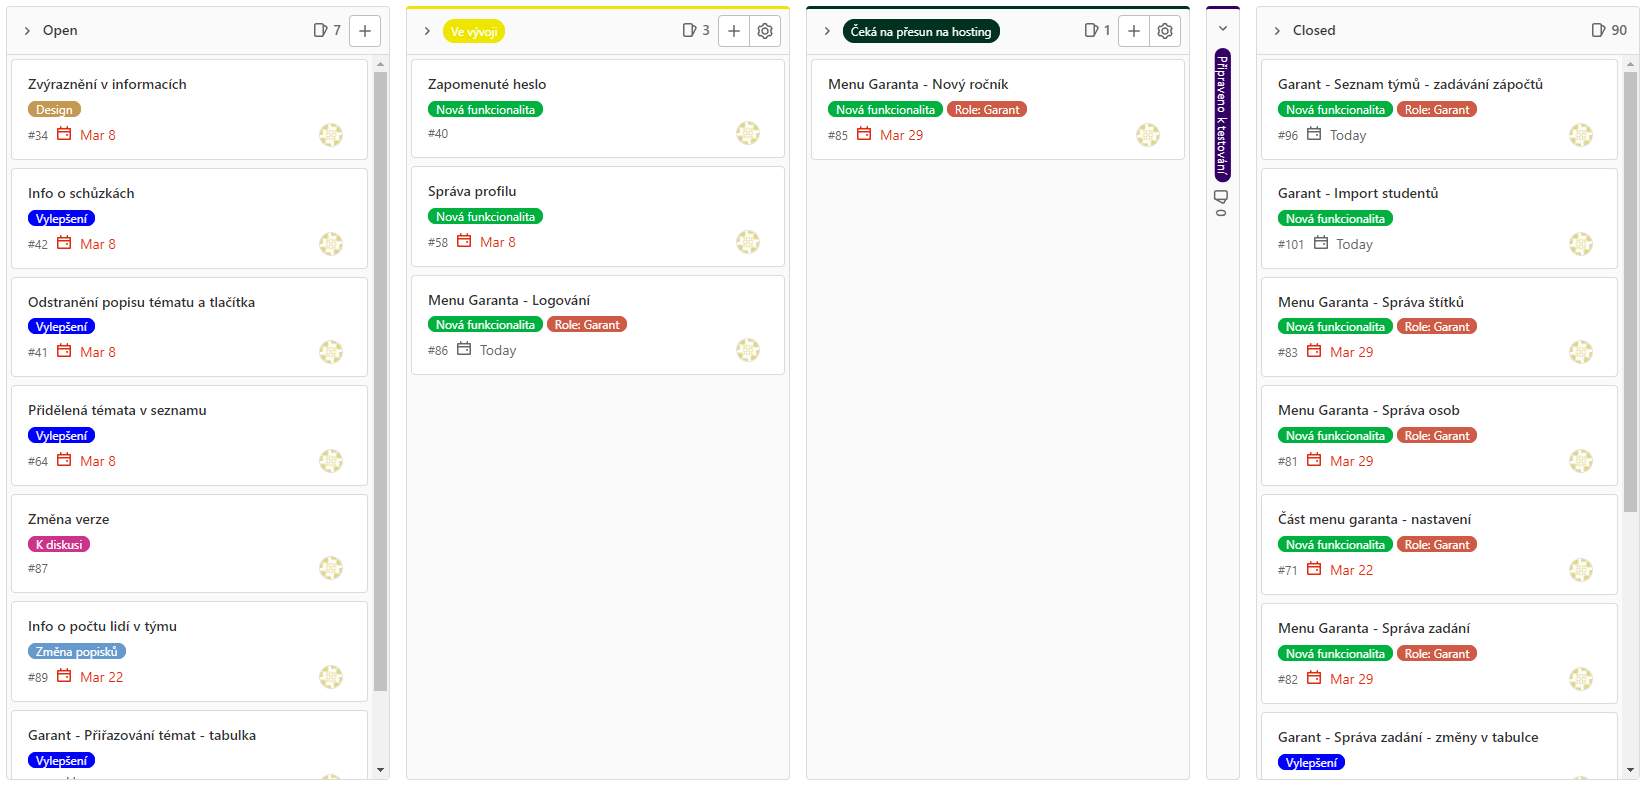
\includegraphics[width=\textwidth]{img/rizeni_projektu/kanban}
		\caption{Ukázka použití tabule s~issues (zdroj: vlastní)}
		\label{fig:kanban}
	\end{figure}
	\par V~informačních technologiích se Kanban používá ve velké míře pro organizaci různých úkolů a požadavků. Různé části vývoje si mezi sebou požadavek vyměňují a tím mění jeho stav.
	\par Například když vývojář dokončí práci na nové funkcionalitě, tak přesune příslušný rámeček ze sloupce \uv{Ve vývoji} do sloupce \uv{Připraveno k~testování}. Tím se tester dozví, že je daný úkol připraven k~testování a může si úkol přiřadit a pracovat na něm.
	\par V~GitLabu je systém Kanbanu implementován v~souvislosti s~issues a jejich štítky. Každý issue je zobrazen jeden rámeček na tabuli Kanban, kam se automaticky po vytvoření issue promítne a po přidělení štítků zařadí do připravených sloupců.
	\par Propojenost s~issue nám ulehčí práci s~přepisováním jednotlivých požadavků do jiných nástrojů, které mají obdobné funkce.
\subsection{MantisBT}
	\par Mantis Bug Tracker je webová aplikace pro nahlašování a evidenci chyb (defektů) nalezených v~průběhu vývoje aplikace. Přidávané defekty lze velmi podrobně popsat, určit prioritu a štítkovat.
	\par MantisBT využíváme pro nahlašování objevených selhání nalezených především, ale ne výhradně pomocí komplexního automatizovaného testování aplikace. Na základě reportování defektů jsou následně žádány jejich opravy chyb a po opravě jsou znovu testovány. Pro naše potřeby používáme vlastní instalaci MantisBT, která je přístupná pro anonymně přihlášené, aby mohli v~budoucnu nahlašovat defekty i uživatelé aplikace.
\chapter{Návrh aplikace}

	\section{Dekompozice specifikace}
		\subsection{Zadání}
		\par V~moment zveřejnění zadání pro mentory je mentorům umožněno zvolit si toto zadání k~mentorování. Po zvolení se automaticky přidělí danému mentorovi.
		\par Po odsouhlasení zadání sborem mentorů se zadání stává tématem, které je možno zveřejnit studentům. Je tedy zobrazováno ve veřejném seznamu témat. Vedoucí týmů mohou o~takové zadání projevit téma hodnotou na pětibodové stupnici vážnosti.\\\\
		Zadání se skládá z~částí:
		\begin{itemize}
			\item název zadání
			\item stručný popis zadání
			\item PDF soubor s~podrobným zadáním
			\item doporučovaná velikost týmu (3--7 lidí)
			\item časová náročnost řešení v~člověkohodinách
			\item kontaktní informace zadavatele
			\item požadovaný profil týmu.
		\end{itemize}
		\par Požadovaný profil týmu obsahuje štítky ze stejného souboru štítků jako v~profilu týmu.
		\subsection{Tým}
		\par Tým je seskupení několika studentů. Má svého vedoucího, který vede tým a hájí jeho zájmy. Cílem týmu je řešení společného projektu na základě přiřazené tématu.
		\par Tým je vytvořen na požádání vedoucího garantem předmětu. Po vytvoření nového týmu se založí nový uživatelský účet pro vedoucího. Následně jsou vedoucímu na jeho studentský email zaslány přihlašovací údaje.
		\par Nastavení týmu provádí zejména vedoucí týmu včetně přidávání studentů do týmu ze seznamu volných studentů zapsaných na předmět.
		\par Vedoucí týmu je zodpovědný za obsah, který do PSTSP vkládá.
		\subsection{Projekt}
		\par Projekt je propojením instance tématu a týmu. Obsahuje dvě základní části. Data o~postupu řešení projektu týmem a informace o~projektu samotném. 
		\par Data o~postupu řešení projektu jsou rozděleny na tři sekce. Plnění minimálních kritérií, plnění postupu projektu a záznamy o~využitých zkušenostech. Všechny záznamy v~těchto sekcích mají dva stavy. Stav, který určil vedoucí týmu a stav, který potvrdil mentor projektu. Na základě potvrzení mentora se určuje opravdový oficiální stav řešení projektu.
		\par Druhá část ohledně údajů o~projektu obsahuje kromě informací o~týmu a samotném tématu vedoucím definované a vyplněné odkazy například na různá úložiště nebo stránky řízení projektu. Dalšími daty jsou údaje o~udělení zápočtů a proběhlých obhajobách.
	\section{Případy užití}
		\par Příklady užití popisují v~krocích způsob používání různých částí aplikace uživatelem nebo systémem. Tyto případy představují se zadavatelem dohodnutou funkčnost systému. Vytvořené případy užití usnadňují tvorbu požadavků na systém pro následné sepsání testovacího plánu.
		\par Z~dílčí specifikace požadavků byly sestaveny případy užití, které popisují práci s~výslednou aplikací. Rozdělení případů užití je ilustrováno v~use-case diagramu (viz obrázek \ref{fig:use-case}). Následuje seznam popsaných případů užití s~popisem funkcí, které pokrývají.
		\subsection{Nepřihlášený uživatel}
			\subsubsection{Přihlášení (UC.01)}
				\par Většina aplikace je přístupná pouze uživatelům dle jejich role. To vytváří potřebu autentizace v~aplikaci. Uživatel má možnost se přihlásit využitím přihlašovací stránky pomocí registrované kombinace přihlašovacího jména a hesla. Pokud je uživatel autentizován, je přesměrován na domovskou obrazovku podle jeho konkrétní role.
			\subsubsection{Zobrazení témat (UC.02--03)}
				\par Nepřihlášený uživatel (např. běžný student) si může zobrazit seznam volných témat v~přehledu, kde se dozví základní informace o~tématech.
				\par Tato témata lze rozkliknout do podrobnější podoby, kde je zobrazen název, stručný popis, časová náročnost, doporučená velikost týmu, zadavatel a mentor tématu. Také lze stáhnout PDF soubor s~podrobným zadáním.
			\subsubsection{Neúplné týmy (UC.04)}
				\par Nepřihlášený uživatel má k~dispozici seznam neúplných týmů, které hledají nové členy. U~každého týmu lze zobrazit seznam obsazených rolí a kontakt na vedoucího týmu.
		\subsection{Přihlášený uživatel}
			\subsubsection{Odhlášení (UC.05)}
				\par Přihlášený uživatel má možnost ukončit svou relaci a odhlásit se. Po této akci je uživatel přesměrován na hlavní stránku nepřihlášeného uživatele.
		\subsection{Vedoucí týmu}
			\subsubsection{Schůzky týmu (UC.06--09)}
				\par Vedoucí týmu může v~aplikaci naplánovat schůzku. Schůzka může obsahovat čas a místo konání a v~jakém uskupení. Schůzka může být například interní, kdy tým se schází s~jeho členy, aby například probrali další postup nebo může být za účasti mentora, zadavatele apod. Pokud je zvoleno, že se schůzky účastní mentor projektu týmu, zobrazí se schůzka kromě stránky týmu i na stránce mentorovaných projektů mentora.
			\subsubsection{Řešení projektu (UC.10--13)}
				\par V~řešení projektu vedoucí týmu zaznamenává postup svého týmu pomocí čtyřstavové hodnoty v~několika kategoriích. Na základě těchto záznamů přiřazený mentor kontroluje a potvrzuje tento postup týmu volbou ze stejného čtyřstavového výběru. Jedná se o~stavy splněno, nesplněno, částečně splněno a nevhodné (pro konkrétní řešení není použitelné).
				\par Vedoucí týmu má na stránce řešení projektu možnost vyplnit a přidat užitečné odkazy.
			\subsubsection{Editace týmu (UC.14--16)}
				\par Vedoucí má možnost přidávat nebo odebírat členy týmu a signalizovat jednotlivé stavy týmu. Členům týmu může přiřazovat a odebírat týmové role. Také může vyplňovat týmový profil z~předem definovaného seznamu schopností. Řádně stanovený profil dle opravdových schopností členů týmu může orientačně pomoci s~výběrem tématu.
			\subsubsection{Stránka tématu a zájem o~téma (UC.17--19)}
				\par Vedoucí, jehož tým nemá přiřazené žádné téma, může na stránce detailu volných témat projevit zájem. Vážnost zájmu o~téma je vybírána ze stupnice pěti hodnot od méně významné po nejvážnější. Vedoucí nemůže projevit zájem o~téma s~vážností, s~kterou již má aktivní zájem o~jiné téma.
				\par Projevené zájmy o~témata jsou zobrazeny na stránce týmu, kde aktivní zájmy může vedoucí odvolat.
		\subsection{Mentor}
			\subsubsection{Změna kontaktních údajů (UC.20)}
				\par Mentor má ve správě profilu zpřístupněnou úpravu kontaktních údajů. Tyto údaje se následně zobrazují například u~detailu zadání, kde je zobrazena \uv{vizitka} přiřazeného mentora.
			\subsubsection{Mentorované projekty (UC.21--25)}
				\par Jednou z~hlavních tabulek mentora jsou mentorované projekty. V~této tabulce uvidí o~každém mentorovaném projektu stav řešení projektu v~kompaktním zobrazení, datum přiřazení tématu týmu a samozřejmě prokliky na projekt a tým.
				\par Předpokládá se, že tato tabulka bude hlavním rozcestníkem mentora v~průběhu mentorování projektů a tedy stránka, na které se nachází, je nastavena jako mentorova domovská stránka.
			\subsubsection{Schůzky (UC.09--10, 26)}
				\par Mentor má přístup k~vytváření schůzek týmů stejně jako vedoucí týmu. Navíc však disponuje tabulkou obsahující schůzky všech týmů, kterých má být mentor zúčastněný.
			\subsubsection{Volba tématu (UC.27--28)}
				\par Součástí navigace mentora je i položka \uv{Témata bez mentora} vedoucí na stránku s~tabulkou témat, která nemají mentora. Tato témata jsou buď zveřejněná pouze pro mentory nebo zcela veřejná. Témata z~této nabídky si mohou mentoři v~detailu zadání přiřadit k~mentorování. Po přidělení je téma z~tabulky odstraněno a naopak se objeví v~tabulce \uv{Témata bez týmu}, pokud téma dosud není přiřazeno žádnému týmu, nebo na stránce \uv{Témata bez týmu}.
			\subsubsection{Témata bez týmu (UC.29--30)}
				\par Stránka témat bez týmu je rozdělena na dvě tabulky. Jedna tabulka obsahuje prostý výčet témat, která má mentor přidělené k~mentorování, ale dosud žádný tým o~ně neprojevil zájem. Druhá komplexnější tabulka obsahuje veškeré projevené zájmy týmu o~zadání. Účel tabulky pochází ze specifikace, kdy mentor posuzuje vhodnost tématu pro daný tým. Výsledek posouzení mentor v~příslušnému zájmu přidělí označení \uv{Nevhodné} nebo \uv{Vhodné}. Výchozí hodnota, kdy mentor dosud není rozhodnut, je \uv{Neohodnoceno}.
			\subsubsection{Historie mentorování (UC.31)}
				\par Aplikace má v~sobě udržovat historii předchozích ročníků TSP. Proto mentor má k~dispozici výpis témat, která dosud mentoroval. Mentor se může na dané projekty prokliknout a prohlížet je.
		\subsection{Garant}
			\subsubsection{Témata bez mentorů (UC.32)}
			\par Garant vidí tabulku se seznamem témat, která nemají dosud přiřazeného mentora. Součástí tabulky je i název zadavatele.
			\subsubsection{Seznam týmů (UC.33--36)}
			\par Obdobná tabulka jako u~pohledu mentora \uv{Mentorovaná témata}, obsahuje tedy seznam projektů s~jejich stavem řešení. Tabulka však navíc obsahuje i týmy, které nemají přiřazené žádné zadání. V~tom případě tak proklik odkazuje na stránku týmu.
			\par Tabulka umožňuje přistoupit k~editaci daného týmu, kde lze upravit údaje o~týmu, zadávat datumy zápočtů a vytvářet záznamy o~obhajobách.
			\subsubsection{Seznam mentorů (UC.37--38)}
			\par Stránka ukazující propojení témat a jejich mentorů mentorů. Proklikem na jméno mentora je mentor zvolen a garant může skrz navigační menu přistupovat k~pohledům mentora.
			\subsubsection{Správa uživatelů (UC.39--41)}
			\par Garant má k~dispozici tabulky se seznamy všech uživatelů, kteří se mohou přihlásit. Tito uživatelé jsou rozděleni dle jejich role na mentory a vedoucí. Garant má oprávnění těmto uživatelům odebrat přístup, čímž jim zamezí v~jejich dalším přihlášení.
			\subsubsection{Správa témat (UC.42--43)}
			\par Garant má přístupnou tabulku všech zadání, kde o~nich může vidět základní informace. 
			\par Součástí správy témat je i vytváření a editace nového zadání. Garant kromě všech dat zadání může přiřadit zadání mentora, určit ročník, ve kterém je zadání vyvěšeno a upravovat jeho viditelnost.
			\subsubsection{Správa štítků (UC.44--48)}
			\par Používané štítky může garant také upravovat, vytvářet nebo znemožnit další použití. V~aplikace jsou dva druhy štítků. Týmové role, které vedoucí přiřazuje členům jeho týmu, a štítky pro profil týmu a tématu. Pokud garant pro jakýkoliv štítek nastaví, že není dostupný pro další užití, není možné jej nově použít. Naopak při znepřístupnění štítku není odebráno již stávající přiřazení, aby nebyla nijak upravována historie již proběhlých projektů.
			\subsubsection{Přidělování témat (UC.49--50)}
			\par Speciální tabulka, kde každý sloupec reprezentuje tým bez přiřazeného tématu a každý řádek jedno volné téma. V~tabulce jsou vyplněné jen ty buňky, kde existuje zájem týmu o~dané zadání. Garant zde vidí vážnost zájmu a datum vytvoření zájmu. Zobrazuje se zde i doporučení mentora, které mentor vyplní na stránce \uv{Témata bez týmu}. Na základě těchto informací garant definitivně přiřadí téma jednomu z~přihlášených týmů.
			\subsubsection{Správa studentů (UC.51--55)}
			\par Na stránce správy studentů má garant k~dispozici tabulku všech přidaných studentů. Z~těchto studentů vedoucí vybírají členy do svých týmů. Garant může nad těmito studenty vyvolávat akce mazání a stanovení vedoucího nového týmu. Při vytvoření nového týmu je potřeba vyplnit počáteční název týmu. Studenti se do této tabulky přidávají buď jednotlivě pomocí formuláře nebo z~přiloženého CSV\footnote{Comma-separated values -- jednoduchý souborový formát pro výměnu tabulkových dat} souboru získaného exportem ze STAGu\footnote{Informační systém studijní agendy}.
			\par Vkládání studenta jednotlivě vyžaduje znalost přihlašovacího jména do systému STAG, křestní jméno, příjmení, email, osobní číslo, ročník ve kterém je TSP studováno a případně obor studia se studovanou fakultou.
			\par Import studentů pomocí CSV umožňuje přidání velkého množství studentů najednou. Jedná se o~vhodnou variantu pro hromadné přidávání studentů například na začátku semestru. Je počítáno s~CSV souborem formátu, který poskytuje systém STAG při exportu studentů zapsaných na daný předmět. I~v~tomto případě je potřeba určit, do kterého ročníku TSP importovaní studenti náleží.
			\subsubsection{Správa ročníků (UC.56--57)}
			\par Garant ve správě ročníků může vidět informace o~jednotlivých proběhlých ročnících. Zároveň může tvořit nové ročníky a nastavovat aktuální ročník TSP. Po zvolení nového aktuální cyklu TSP se původní cyklus považuje za historický a je tak i zobrazován ve zbytku aplikace. Tímto způsobem je řešeno zachování předchozích ročníků TSP, kdy v~běžném stavu aplikace se zobrazují zejména údaje vztažené k~aktuálnímu ročníku TSP.
			\subsubsection{Logování (UC.58--59)}
			\par Pro sledování správné činnosti aplikace má garant přístup k~zobrazení logovacích záznamů. Tato funkce je zprostředkována pomocí parsování sekvencí záznamů do tabulky. Garant si může zvolit logovací soubor k~nabídky k~jednoduchému zobrazení. Zvolený záznam může také stáhnout v~textové podobě a provádět s~ním další operace.
		\begin{figure}[h]
			\centering
			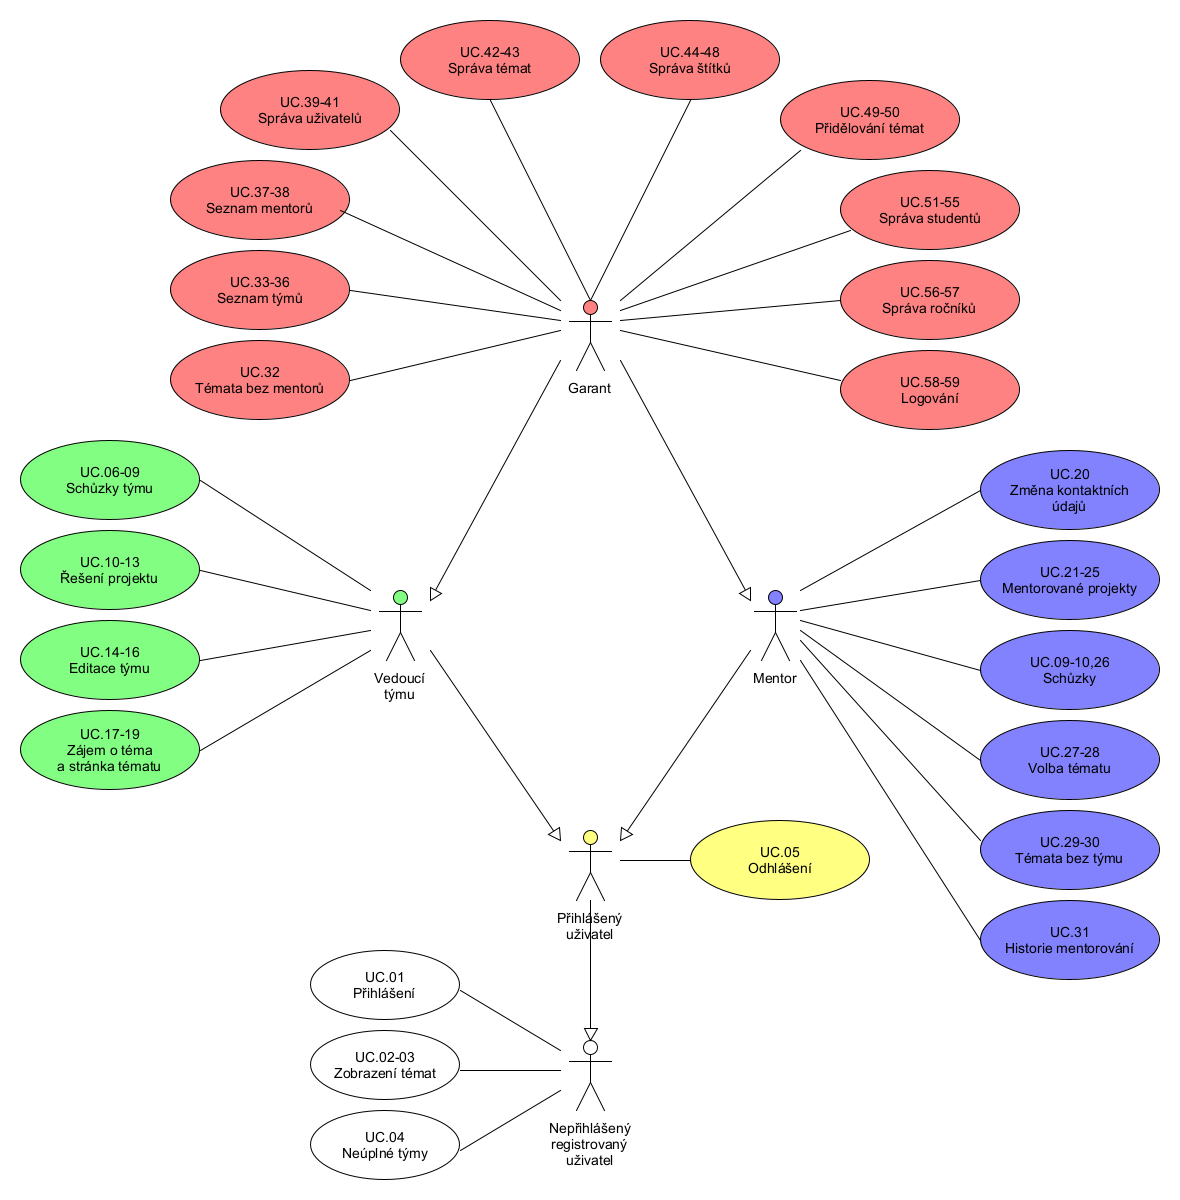
\includegraphics[width=0.8\textwidth]{img/use_case/use_case_diagram}
			\caption{Schéma případů užití (zdroj: vlastní)}
			\label{fig:use-case}
		\end{figure}
	\chapter{Architektura aplikace}
		\section{Třívrstvá architektura}
		\par Architektura MVP\footnote{Model-View-Presenter -- třívrstvá architektura} je třívrstvový návrh struktury aplikace pro rozdělení souborů dle funkčnosti s~ohledem na rozšiřitelnost. MVP architektura se skládá z~datové části (model), která se stará o~práci s~daty a umožňuje vytvářet abstrakci nad jednotlivými strukturami. Například jednotlivé akce s~databází v~kontextu dat, se kterými aplikace pracuje. Další část je aplikační vrstva (presenter), která řídí chod aplikace, předává data z~šablon do modelů a naopak. Poslední vrstvou je vrstva prezentační (view). Ta se skládá z~jednotlivých šablon a prezentace dat. Představuje tak rozhraní, přes které uživatel komunikuje s~aplikací.
		\par Mezi další velice rozšířenou architekturou patří MVC architektura, ze které MVP struktura vychází. Hlavním rozdílem mezi MVP a MVC architekturami je způsob zpracovávání vstupů od uživatele \cite{3Vrstvy}.
		\par Rozdělení aplikace do několik vrstev je výhodné z~důvodu nezávislosti jednotlivých částí. To zvyšuje efektivnost vývoje, kdy jednotlivé části aplikace mohou být vytvářeny téměř nezávisle.
		
		\section{Komponenty aplikace v~Nette}
		\par Komponenty jsou části aplikace, které vkládáme do stránek. Nejčastěji se jedná o~formuláře, tabulky a další objekty, které je možné používat opakovaně.
		\par Nette má v~sobě vestavěný komponentový systém, který umožňuje komponenty vkládat na stránky a někdy dokonce do jiných komponent, kdy se tak tvoří tzv. komponentový strom. Velkou výhodou je, že se komponenta tvoří až tehdy, kdy je opravdu použita. To představuje výhodu zejména při zpracování AJAX požadavků, kde je typicky výsledkem operace pouze část stránky, kdy není komponenta využita. Díky tomu se vůbec nevytváří a tím se šetří výkon serveru.
		\par Komponenty se vytvářejí v~továrních funkcích v~presenteru. Tyto funkce mají prototyp \texttt{createComponent<Name>(): Control} \cite{NetteComponents}.
		
		\subsection{Ukázka tovární metody v~presenteru}
		\begin{lstlisting}[caption={Ukázka tovární metody v~presenteru}]
class DefaultPresenter extends Nette\Application\UI\Presenter
{
	protected function createComponentPoll(): PollControl
	{
		$poll = new PollControl;
		$poll->items = $this->item;
		return $poll;
	}
}
\end{lstlisting}
		
		\par Komponentu lze definovat přímo v~tovární metodě, ale pro účely znovupoužitelnosti je možné pro komponentu vytvořit vlastní třídu dědící třídu \texttt{Nette\textbackslash Application\textbackslash UI\textbackslash Control}.
		
		\section{Dependency Injection v~Nette}
		\par Vkládání závislostí je technika programování vedoucí k~čistému a přehlednému kódu. Princip tohoto způsobu programování spočívá v~předávání zdrojů (služeb), které konkrétní funkce nebo třída vyžaduje, aby splnila svoji úlohu. Cílem je zamezit získávání zdrojů přímo v~daném objektu, kdy programátor bez dodatečné informace neví s~jakými zdroji informací systém pracuje a jak je případně získává. V~těchto případech říkáme, že se vytváří v~aplikaci skryté vazby, díky kterým vzniká nepřehledný a špatně udržitelný kód \cite{PHP-DI}.
		\par Pro implementaci DI se využívá tzv. Dependency Container. Tento nástroj slouží k~uchování instancí jednotlivých služeb a jejich vytváření, pokud se jedná o~závislosti aktuálně potřebných částí aplikace.
		\par Nette pro implementaci Depencency Containeru využívá vlastní knihovnu Nette DI Container. Knihovna se stará o~automatické generování a aktualizaci tříd kontejneru na základě konfiguračního souboru formátu NEON. Díky této technologii programátor nemá potřebu implementace vlastního řešení a může se soustředit na vývoj logiky aplikace. Při vytváření jednotlivých služeb však nesmí zapomenout tuto službu zaregistrovat zapsáním do konfiguračního souboru.
		\par Další technologií, kterou Nette využívá, je nástroj Autowire. Ten se stará o~automatické předávání závislostí z~dependency kontejneru do konstruktorů a parametrů dalších funkcí \cite{NetteDI}.
		
		\section{Formuláře v~Nette}
		\par Formuláře jsou důležitou součástí webového systému. Jedná se o~jednu z~možností jak získat uživatelský vstup. Zároveň ale představují bezpečnostní riziko, které je nutno ošetřit. Typů útoků skrz uživatelský vstup přes formuláře je velké množství a jejich ošetření klade nemalé časové a znalostní nároky na programátora. Také i proto je tvorba a validace formulářů velmi rutinní činnost. Framework Nette proto přichází se svým řešením Nette Forms. Jedná se o~možnost tvorby formulářů, kdy programátor definuje základní prvky formuláře a framework sám z~těchto informací sestaví formulář. Výhoda tohoto přístupu spočívá v~bezpečnosti. Nette Forms totiž validuje vstupy uživatele podle definovaných validačních pravidel a to jak na straně backendu, tak v~případě připojených příslušných JavaScript skriptů i na straně frontendu. Aplikaci tedy komponenta vrátí validovaná data, která může bez starostí použít.
		\par Tvorba formuláře probíhá jako použití obyčejné komponenty. Tovární funkce vrací instanci třídy \texttt{Nette$\backslash$Application$\backslash$UI$\backslash$Form}. Funkce instanci vytvoří a postupně do ní přidává formulářové prvky, kterým lze definovat další různá pravidla nebo vlastnosti. Je také potřeba implementovat kód, který se spustí po nějaké události ve formuláři. Zejména je myšlena událost úspěšně odeslaného formuláře, kdy je pravděpodobně nutné vykonat nějakou akci aplikace (např. uložit data).
		\par Vytvořenou komponentu formuláře je možno automaticky vykreslit dle předem vytvořené šablony pomocí šablonovacího systému Latte a tak jednoduše vložit formulář do příslušné stránky. Je však ponechána možnost vytvoření si jednotlivých formulářových prvků v~šabloně a dle identifikátoru je propojit s~prvky v~komponentě \cite{NetteDI}.
		
		\section{Database Explorer}
		\par Vyvíjená aplikace je postavená na předávání dat mezi aplikací a databází. Proto je využita služba Nette Database Exploreru, který umožňuje vytvářet dotazy databáze bez potřeby psát kompletní SQL příkazy. Je zde využíváno techniky objektově relačního mapování, kdy není výsledkem dotazu pole hodnot, ale objekty, nad kterými lze volat další funkce (viz ukázka kódu \ref{lst:DBExplorer}).
		\begin{minipage}{\linewidth}
		\begin{lstlisting}[language=PHP, caption={Ukázka použití Nette Database Explorer},label={lst:DBExplorer}]
$user = $explorer->table('USER')->get($id);
$address = $explorer->table('ADDRESS')->where('id', $user->id)->fetch();
$address->update([
	'street' => 'New Street',
	'city' => 'City',	
]);
\end{lstlisting}
\end{minipage}
		\par Databáze nám vrací objekt typu \texttt{ActiveRow} reprezentující záznam výsledku dotazu nebo \texttt{Selection} představující výběr. Pomocí instancí typu \texttt{ActiveRow} lze přistupovat k datům jednotlivých sloupců záznamu. Naproti tomu u objektu \texttt{Selection} je jeho hlavním účelem možnost iterování přes záznamy a získat tak instance \texttt{ActiveRow}. 
		\par Použití Database Exploreru poskytuje nativně i ochranu proti různým typům útokům zejména před SQL Injection. Zároveň se za programátora snaží prvotně optimalizovat dotazy pro zvýšení efektivnosti a tím i rychlosti.
		
		\section{Testovatelnost aplikace}
		\label{sec:testovatelnost}
		\subsection{Testování pomocí Selenia}
		\par Aby bylo možné aplikaci automaticky otestovat je potřeba umožnit testovacímu softwaru ovládat aplikaci. Proto musí být veškeré ovládací prvky jednoznačně identifikovatelné. Toho docílíme zavedením jednoznačných identifikátorů vložených do atributu \texttt{id} daných elementů.
		\par Selenium je díky tomu schopno nalézt požadovaný prvek stránky. Takto jednoznačně identifikovatelné není potřeba mít pouze akční prvky typu odkazu nebo tlačítka, ale také i další prvky stránky. Ty Selenium potřebuje nalézt, aby z~nich mohl číst data.
		\par Navržené automatické testování se na tuto vlastnost spoléhá např. při orientaci v~aplikaci. Každá stránka s~obsahem má svůj nadpis. Tento nadpis má jednoznačný identifikátor v~celé aplikaci. Na základě této značky se při testování zjišťuje, zda je otevřena žádaná stránka. Obdobným způsobem dokáže také získat data z~jednotlivých elementů, ke kterým se dostane, a může provést jejich kontrolu.
		
		\subsection{Jednotkové testování}
		\par Princip jednotkového testování je ověření nejelementárnějších procedur aplikace. V~tomhle ohledu se činnost vyvíjené webové aplikace skládá z~většinové části pouze z~interpretace dat z~a do databáze voláním funkcí Nette frameworku. Tak se nedostáváme na elementární úroveň, kterou můžeme jednotkově testovat. Avšak při vývoji byly vytvořeny pomocné procedury, které pomáhají se zpracováním dat (např. parsování). Tyto funkce jsou oddělené od logiky aplikace a jsou závislé pouze na svých vstupech. Pro těchto několik funkcí byly vytvořeny jednotkové testy, které ověřují jejich výstupy.
		
		\subsection{Logování}
		\par Logování je určené pro dlouhodobé sledování činnosti programu. V~sekvenci záznamů je možné dohledat souvislosti zpracovaných akcí a stavu systému. Pomocí logování sledujeme zejména běžnou činnost programu, výskyt chyb a výjimek, konfiguraci programu a její změny. Tato technika může být použita i pro ladění, ale v~našem případě máme jiné ladící nástroje \cite{OKSPrednasky}.
		\par Pro PHP existuje profesionálně používaná knihovna Monolog\footnote{https://github.com/Seldaek/monolog}. Ta je již integrována do známých frameworků jako Symfony, Laravel i Nette. Logovací záznam je pole o~jednotlivých položkách např. úroveň, časové razítko, jméno loggeru, zaznamenávaná zpráva, dodatečné informace, atd. Tyto údaje však negeneruje programátor přímo, ale zpravidla pomocí logovacích funkcí loggeru.
		\par Záznamy loggerů ukládáme do adresáře \texttt{/log/syslog/} v~textovém formátu \texttt{.log}. Záznamy jsou rozděleny do jednotlivých souborů dle dne. Veškeré tyto a další parametry lze změnit v~konfiguraci aplikace a upravit tak logování dle zjištěných reálných potřeb systému.
		
		\section{Vícejazyčnost}
		\par Mezi požadavky na aplikaci je podpora vícejazyčného prostředí. Zejména byla vyžádána možnost přepnout rozhraní do anglického jazyka.
		\par Pro splnění tohoto požadavku byl implementován balíček pro implementaci překladů \texttt{kdyby/translation}. Balíček umožňuje vkládat do šablon a kódu řetězce dle jejich identifikátoru ze souborů s~překlady. Vždy se tak použije řetězec ze souboru dle aktuálně nastaveného jazyka.
		\par Soubory s~překlady jsou uloženy ve formátu NEON ve vlastním adresáři. Každé jazykové podání je obsaženo v~samostatném souboru. Hodnoty jednotlivých překladů jsou uspořádány v~hierarchické struktuře. Pro vizuální i logické oddělení tak lze větvit strukturu dle částí aplikace, ve kterých jsou překlady řetězce obsaženy.
	
	\section{Databázová struktura}
		\par Struktura databáze musí obsahovat veškeré informace použitelné v~PSTSP a umožnit jejich snadné propojení. Dalších aspektem pro tvorbu struktury je použitý PHP framework, který využívá službu pro správu databázových dotazů a jejich optimalizaci. Pro jeho správnou funkci je potřeba mít strukturu databáze řádně připravenou včetně vytvořených indexů a propojení pomocí cizích klíčů.
		\par Databázová struktura musí respektovat, že požadavkem na aplikaci je prohlížení historie. To nás přivádí na strategii, že každá tabulka u~které to bude potřeba bude provázána s~tabulkou \texttt{PERIOD} jejíž řádky představují jednotlivé ročníky TSP. Také se však vyskytuje problém u~odstraňování záznamů. Prakticky nebude možné z~databáze cokoli odstraňovat, aby nebyl porušen konzistentní stav již proběhlých projektů. To je následně ve struktuře zapracováno v~různých tabulkách sloupcem s~příznakem, který určuje zda je prvek odstraněn nebo znepřístupněn pro další užití. Tím prvek stále existuje, není porušeno integritní omezení a potřebné změny pro nové projekty jsou upraveny.
		\par Podle požadavků byl sestaven následující model 23 tabulek, jejichž strukturu lze vidět v~diagramu (viz obrázek \ref{fig:strukturaDB}).
		
		\begin{figure}[H]
			\centering
			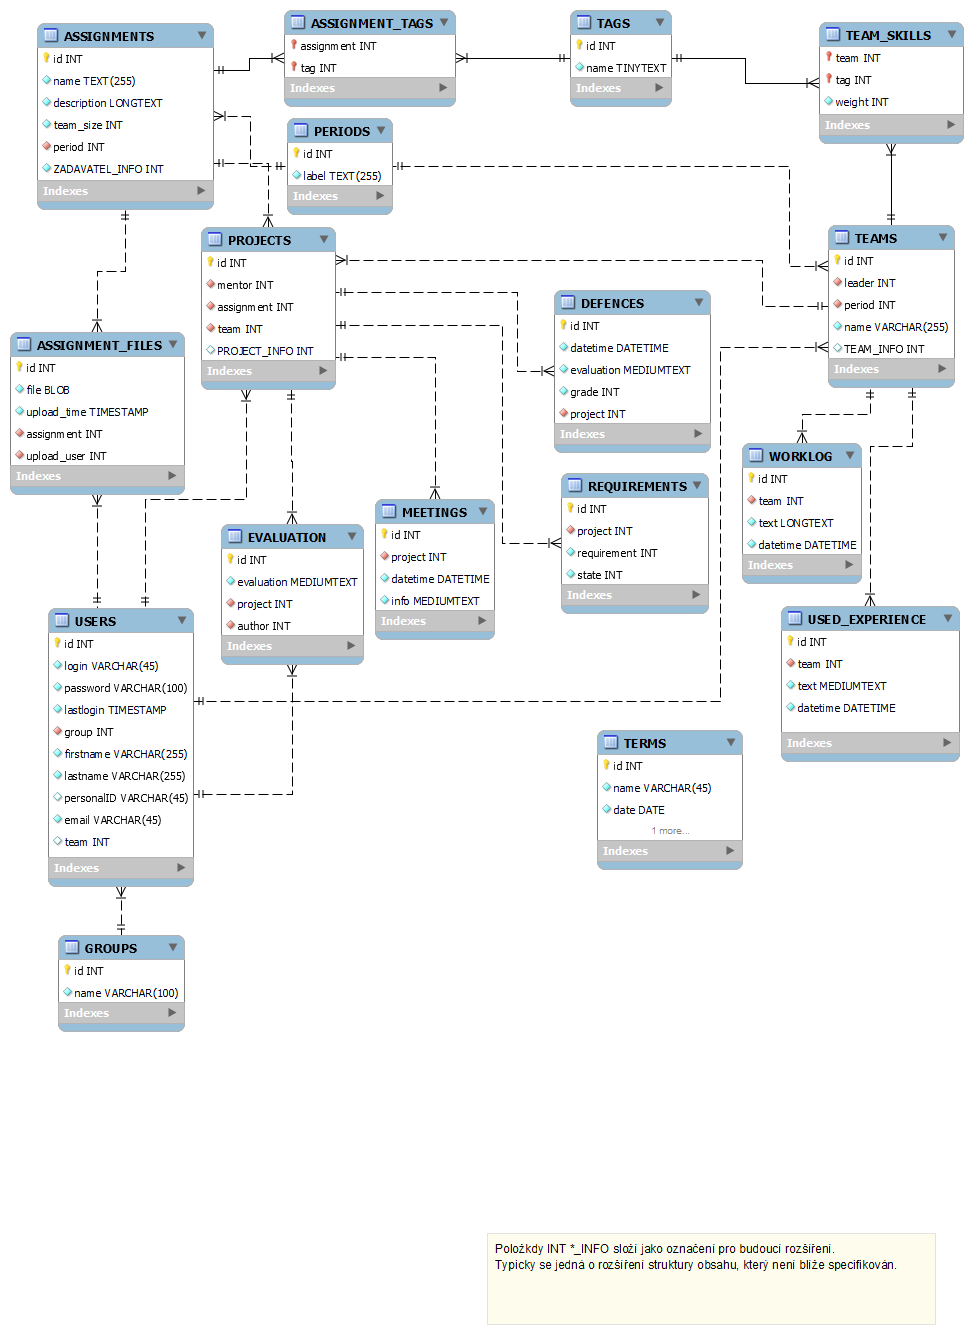
\includegraphics[width=0.8\textwidth]{img/database/database_model}
			\caption{Schéma databázové struktury (zdroj: vlastní)}
			\label{fig:strukturaDB}
		\end{figure}
		\subsection{Základní tabulky}
			\begin{itemize}
				\item \texttt{USER} -- tabulka pro ukládání uživatelů, kteří mají/měli přístup do aplikace. Součástí této tabulky jsou přihlašovací údaje, role uživatele a následné propojení na další informace dle role uživatele.
				\item \texttt{STUDENT} -- uživatelé s~rolí \uv{Vedoucí} vycházejí ze záznamu tabulky \texttt{STUDENT}, která obsahuje seznam všech studentů studujících předměty TSP.
				\item \texttt{TEAM} -- tabulka pro evidenci týmů s~jejich vedoucích.
				\item \texttt{PROJECT} -- tabulka propojuje zadání z~tabulky \texttt{ASSIGNMENT} a týmu z~tabulky \texttt{TEAM}, tím vzniká projekt.
				\item \texttt{CONTACT} -- tabulka pro evidenci informací a kontaktů na mentory a zadavatele.
				\item \texttt{ASSIGNMENT} -- tabulka pro ukládání jednotlivých zadání.
				\item \texttt{ASSIGNMENT\_INTEREST} -- tabulka pro evidenci zájmů o~témata.
				\item \texttt{MEETING} -- tabulka pro evidenci schůzek týmů
			\end{itemize}
		\subsection{Číselníkové tabulky}
		\par Tabulky sloužící jako číselník.
		\begin{itemize}
			\item \texttt{TEAM\_ROLE} -- tabulka dostupných rolí v~týmu
			\item \texttt{TAG} -- tabulka profilů pro použití v~týmu a zadání
			\item \texttt{PROGRESS} -- tabulka se seznamem bodů, které tým v~projektu plní
			\item \texttt{REQUIREMENT} -- tabulka se seznamem kritérií, která musí tým splnit
			\item \texttt{EXPERIENCE} -- tabulka využitých zkušeností
			\item \texttt{PERIOD} -- tabulka jednotlivých ročníků aplikace a předmětů TSP
			\item \texttt{ROLE} -- tabulka dostupných rolí uživatelů aplikace
		\end{itemize}
		\subsection{Spojovací tabulky}
			\par Následující tabulky jsou pomocné tabulky pro realizaci N:M relace. Propojují typicky dvě tabulky s~případným ohodnocením nebo informacemi dané relace.
			\begin{itemize}
				\item \texttt{TEAM\_ROLE\_STUDENT} -- propojení tabulek \texttt{TEAM\_ROLE} a \texttt{STUDENT}. Tabulka slouží pro zaznamenání přiřazení rolí jednotlivým členům týmu.
				\item \texttt{TEAM\_SKILL} -- propojení tabulek \texttt{TAG} a \texttt{TEAM}. Tabulka specifikuje jednotlivé profily týmů.
				\item \texttt{ASSIGNMENT\_TAG} -- propojení tabulek \texttt{TAG} a \texttt{ASSIGNMENT}. Tabulka specifikuje jaký profil týmu je předpokládán pro tým, který bude zadání řešit.
				\item \texttt{PROGRESS\_STATE} -- propojení tabulek \texttt{PROGRESS} a \texttt{PROJECT}. Tabulka eviduje postup v~řešení projektu. Relace uchovává stavovou hodnotu daného přepínače.
				\item \texttt{REQUIREMENT\_STATE} -- propojení tabulek \texttt{REQUIREMENT} a \texttt{PROJECT}. Tabulka eviduje plnění kritérií při řešení projektu. Relace uchovává stavovou hodnotu daného přepínače.
				\item \texttt{EXPERIENCE\_STATE} -- propojení tabulek \texttt{EXPERIENCE} a \texttt{PROJECT}. Tabulka eviduje stav potvrzení využitých zkušeností. Relace uchovává stavovou hodnotu daného přepínače.
			\end{itemize}
		\subsection{Další tabulky}
			\begin{itemize}
				\item \texttt{ASSIGNMENT\_FILE} -- Tabulka sloužící pro uložení PDF souborů s~příslušnými informacemi.
				\item \texttt{SETTING} -- Tabulka s~nastavením aplikace. Každý záznam představuje typ nastavení a jeho hodnotu.
			\end{itemize}
	\section{Uživatelské rozhraní}
	\par Důležitou částí aplikace je uživatelské rozhraní. Pomocí něj je totiž aplikace ovládána a jedná se o~pohled, kterým uživatel pracuje s~aplikací. Zjednodušeně lze říct, že nekvalitně vytvořené uživatelské rozhraní může ohrozit příjemný uživatelský zážitek z~používání aplikace a znepříjemnit práci se systémem. Návrhu uživatelského prostředí je tedy potřebné věnovat značnou pozornost.	
	\par Návrh rozhraní rozděluje zobrazovací prostor na tři hlavní části. Horizontální navigační lišta, která obsahuje hlavní rozcestník na důležité stránky vztahující se k~předmětu (např. CourseWarová stránka předmětu), údaje o~přihlášeném uživateli a nastavení jazykové předvolby. Tato navigace je navržená tak, že je vždy přístupná. Pod ní se zobrazují hlášky aplikace například o~úspěšně provedených akcích. Na levé straně straně zobrazovací plochy je umístěna hlavní (vertikální) navigace systému. Obsahuje odkazy na stránky, ke kterým má aktuální uživatel přístup. Poslední a hlavní částí je část obsahu, která zobrazuje obsah jednotlivých stránek. Tato stránka pro orientaci v~aplikaci vždy obsahuje i název stránky.
	\par Při návrhu je potřeba klást důraz na jednotnost. Uživatel by měl mít shodný způsob používání napříč aplikací.
	
	\subsection{Responzivita}
	\par Responzivní desing spočívá v~přizpůsobení zobrazení obsahu šířce okna webového prohlížeče (příp. velikosti obrazovky zařízení). To znamená, že uživatel navštěvující stránku ze stolního počítače nebo mobilního zařízení uvidí uspořádaný obsah tak, aby byl na daném zařízení dostatečně čitelný a ovladatelný \cite{CSSOkamzite}.
	\par Front-end aplikace je implementován frameworkem AdminLTE, který staví na základech technologie Bootstrap. Díky tomu je snadné udržovat v~aplikaci responzivní design, pokud je dodržena správná HTML struktura a jsou důsledně aplikovány styly použitím tříd stylů. 
	\par V~aplikaci jsou jednotlivé celky umístěné do tzv. karet. Díky tomu je možné je snadno přemisťovat jako ucelené balíčky uspořádané do sloupců a řádků. Například při zobrazení na malém mobilním zařízení jsou veškeré karty uspořádány do jednoho sloupce, kdy je podstatné, aby ty důležitější karty byly zobrazovány navrchu.  
	\section{Návrh loga}
	\par Aplikace pro svoji vizuální komunikaci a rozeznatelnost potřebuje logo.
	\par Vývoj loga vychází z~názvu projektu \uv{Podpůrný software TSP} respektive z~jeho zkratky \uv{PSTSP}. Bylo využito skutečnosti, že zkratka názvu je palindromem\footnote{Palindrom je slovo, které lze číst zleva i zprava stejně}, a vlastnosti osové souměrnosti písmena \uv{T}.
	\par Počáteční návrh loga (viz obrázek \ref{fig:logo.prvni_navrh}) spočívá v~zrcadlení části \uv{PS} resp. \uv{SP}, které jsou \uv{zastřešeny} velkým písmenem \uv{T}, kdy jeho vertikální čára působí jako zrcadlo.
	\par Finální verze (viz obrázek \ref{fig:logo.final}) vychází z~prvotního návrhu. Celé logo bylo vloženo do šestiúhelníkového rámu s~přidanou perspektivou. Písmena k~sobě přiléhají a kvůli tvarům písmen a rámu jsou hranaté. Barevná paleta byla vybírána s~ohledem na barvy univerzity (modrá) a fakulty (zlatá). V~celkovém pojetí logo připomíná výraznou šipku symbolující posun se zlatavým ohonem a bílým vzduchem. Logo tedy symbolizuje rychlý pokrok vpřed.
	\begin{figure}[H]
		\centering
		\begin{minipage}[c]{0.4\linewidth}
			
\includegraphics[width=1\textwidth]{img/logo/prototype_logo}
			\caption{Prvotní návrh loga (zdroj: vlastní)}
			\label{fig:logo.prvni_navrh}
		\end{minipage}\hfill
		\begin{minipage}[c]{0.4\linewidth}
			
\includegraphics[width=1\textwidth]{img/logo/transparent_bg_logo}
			\caption{Finální verze loga aplikace (zdroj: vlastní)}
			\label{fig:logo.final}
		\end{minipage}
	\end{figure}
	\subsection{Použití loga}
	\par Logo je plánováno pro použití v~samotném systému a hlavně pro použití jako favicon webové aplikace.
	\par Otázka ikon webových stránek není úplně triviální, protože je potřeba definovat jednotlivé obrázky a další údaje pro různé velikosti zobrazení na různých platformách. Typický příklad je ikonka v~prohlížeči, kde se použije rozlišení 64$\times$64 px, na rozdíl od mobilního telefonu s~moderním operačním systémem s~ikonkou stránky na ploše, kdy se použije podstatně větší rozlišení s~definovanou barvou pozadí.
	\par Pro vyřešení této otázky byl nalezen a použit nástroj RealFaviconGenerator\footnote{Dostupné na https://realfavicongenerator.net/}, který z~jednoho vstupního obrázku umožní sestavit si vlastní nastavení faviconů pro různé platformy. Výsledkem tohoto procesu jsou prvky HTML hlavičky, které stačí implementovat do práce. 
	\par Díky tomuto nástroji máme rychle zajištěnou kompatibilitu zobrazení ikonky webu.
\chapter{Realizace}
	\par Během realizace byly využívány postupy a technologie uvedené v~předchozích kapitolách.
	\section{Adresářová struktura}
	\par Adresářová struktura vychází z~třívrstvé MVP architektury a \uv{best practices} použití Nette Frameworku.
	\par Struktura adresářů je naznačena v~následujícím stromu:
	\dirtree{%
		.1 /.
		.2 app.
			.3 components \normalfont{-- třídy znovupoužitelných komponent}.
			.3 locale \normalfont{-- překlady}.
			.3 Model \normalfont{-- třídy modelů}.
			.3 Presenters \normalfont{-- třídy presenterů}.
				.4 templates \normalfont{-- soubory šablon a pohledů}.
			.3 Router \normalfont{-- konfigurace URL adres}.
			.3 Bootstrap.php \normalfont{-- zaváděcí třída Bootstrap}.
		.2 config \normalfont{-- konfigurační soubory}.
		.2 log \normalfont{-- logovací soubory}.
		.2 temp \normalfont{-- dočasné soubory, cache}.
		.2 tests \normalfont{-- třídy s~jednotkovými testy}.
		.2 vendor \normalfont{-- knihovny instalované Composerem}.
			.3 autoload.php \normalfont{-- automatické načítání nainstalovaných balíčků}.
		.2 www \normalfont{-- veřejný adresář}.
			.3 src \normalfont{-- CSS a JavaScript soubory}.
			.3 index.php \normalfont{-- prvotní soubor, kterým se aplikace spouští}.
	}

	\section{Konfigurace aplikace}
	\par Framework Nette používá konfiguraci pomocí externích souborů formátu NEON. Zápis konfigurace je velmi podobný zápisu ve formátu YAML.
	\subsection{Konfigurace databázového spojení}
	\par Na databázi se aplikace připojuje nativním připojením v~Nette pomocí balíčku \texttt{nette/database}, kdy spojení získáme jako službu z~DI kontejneru.
\begin{minipage}{\linewidth}
		
	\begin{lstlisting}[caption={Konfigurace databázového spojení},label={lst:spojeniDB}]
database:
	dsn: 'mysql:host=127.0.0.1;dbname=test'
	user: root
	password: password
\end{lstlisting}
\end{minipage}
	\par V~nastavení databázové struktury (viz ukázka kódu \ref{lst:spojeniDB}) nastavujeme položku \texttt{dns} jako textový řetězec obsahující typ připojované databáze, adresu serveru (případně s~číslem služby) a název výchozího zvoleného schématu v~databázi. Dále se nastavuje uživatelské jméno a heslo pro připojení.
	\subsection{Vlastní nastavení aplikace}
	\par Do konfigurace aplikace lze vkládat vlastní konfigurovatelné možnosti, které lze následně v~aplikaci načítat a upravovat tak chování systému. V~konkrétním případě tohoto využíváme pro nastavení režimu pro testování aplikace, kdy veškerá emailová komunikace se zasílá na předem definovaný email (viz ukázka kódu \ref{lst:nastaveni-test}).
		\begin{lstlisting}[caption={Konfigurace testovacího režimu},label={lst:nastaveni-test}]
parameters:
	config:
		testing:
			enabled: true
			
			databaseResetFileName: 'testDatabase.sql'
			
			testMail: true
			testMailAddress: 'hintik@hintik.cz'
			# testMailAddress: 'schooltestforsmtp123@gmail.com'
			
			testPassword: true
			testPasswordValue: 'tsp'
		\end{lstlisting}
	\section{Vylepšování aplikace}
	\par Již implementované funkce jsou v~aplikaci stále vylepšovány. Nejčastěji z~důvodu nalezených defektů a následujících případech.
	\subsection{Úpravy dle aktualizování specifikace}
	\par V~průběhu vývoje byla specifikace a požadavky několikrát upravovány. To vyžadovalo obvykle úpravy na již dokončených částí aplikace. Aktualizace specifikace pramenily většinou z~diskusí garantů předmětu a budoucích mentorů, kteří následně přehodnotili postoje k~původně požadovaných funkcím. 
	\subsection{Připomínky budoucích uživatelů}´
	\par Od počátku vývoje jsou přijímány podměty pro vylepšování uživatelského komfortu z~používání aplikace. Nejčastěji se jednalo o~úpravy vzhledu, popisků nebo změnu pozicování prvků stránek. Vyskytly se však návrhy na přidání zcela nových funkcionalit, které vytváří zcela nový modul aplikace nebo pouze rozšiřují již existující funkce.
	\par Na začátku prosince roku 2021 bylo uskutečněno představení vyvíjeného softwaru budoucím mentorům předmětů TSP za účelem získání zpětné vazby od reálných budoucích uživatelů tohoto systému.
	\par Veškeré návrhy a podměty byly projednány a případně zaneseny do nástrojů pro řízení projektu.
	\section{Požadavky na zavedení aplikace}
	\par Pro úspěšnou instalaci projektu na webovém serveru je potřeba splnit požadavky pro běh programu. Nejdůležitější požadavek pro spuštění je mít nainstalovaný webový server s~modulem PHP podporující verzi PHP minimálně 7.2. Další požadavky se shodují s~požadavkami frameworku Nette ve verzi 3.1. Nette však již spolehlivě běží na každé běžné PHP instalaci a zrušil tedy nástroj Requirement Checker.
	\par Případné balíčky aplikací jsou př¨ibalené s~aplikací nebo je lze získat pomocí nástroje Composer a přiložené definice závislostí.
	\par Dále je také požadována přístupná databáze MySQL nebo MariaDB pro trvalé úložiště dat.
	\par Pro korektní odesílání emailových zpráv je potřeba také definovat SMTP server, přes který se má korespondence odesílat.
	\pagebreak
	\section{Výsledná aplikace}
	\par Aplikace byla vyvinuta do verze 0.9. Tato verze již poskytuje dostatečné funkce pro konání prvního ročníků předmětů TSP. Funkce \uv{Ročníky} není plně implementována a nyní aplikace zobrazuje informace nezávisle na aktuálně zvoleném ročníku. Funkce vícejazyčnosti je připravena. U~vícejazyčnosti je potřeba pouze vytvořit soubory s~překlady a nahradit jimi aktuálně vložené řetězce přímo do šablony.
	\subsection{Verze 1.0}
	\par Vývoj nadále bude pokračovat s~cílem dokončit implementaci nedokončených funkcionalit, vylepšení vzhledu a responzivity.
	\par Verze 1.0 by měla představovat již zcela hotovou aplikaci pro organizaci předmětů TSP i v~následujících ročnících. S~touto verzí je počítáno s~nasazením na univerzitním serveru, kde bude produkční verze aplikace poskytována pro účely organizace výuky.
	\section{Ukázky vybraných částí aplikace}
	\par V~následující sekci jsou představeny kritické části aplikace, které jsou důležité pro základní funkci aplikace.
	\subsection{Rozhraní}
	\par Rozhraní a celkový vizuál aplikace je tvořen frontendovým frameworkem AdminLTE. Celý vzhled tak vychází z~ukázek\footnote{https://adminlte.io/themes/v3/} použití tohoto frameworku.
	\subsubsection{Navigace}
	\par Společnou částí aplikace jsou navigační panely. Postranní navigační panel obsahuje položky dle role aktuálního uživatele (viz obrázek \ref{fig:example_nav}).
	 \begin{figure}[H]
	 	\centering
	 	
\includegraphics{img/ukazky/navigace}
	 	\caption{Ukázka navigace mentora (zdroj: vlastní)}
	 	\label{fig:example_nav}
	 \end{figure}
 	\subsubsection{Alerty}
 	\par Uživatel je po každé akci, která upravuje data, informován vyskakujícím okénkem (viz obrázek \ref{fig:example_alert}) obsahují zprávu o~úspěšnosti akce. Tato komponenta je důležitá pro informovanost uživatele a také napomáhá k~testování aplikace. Při testování se jedná o~jeden z~posuzujících se o~úspěšnosti vykonané operace. Pro důvody testování okénko samovolně nezmizí a je potřeba ho zavřít kliknutím na křížek.
 	\begin{figure}[H]
 		\centering
 		
\includegraphics{img/ukazky/alert}
 		\caption{Ukázka alertu po vykonané akce (zdroj: vlastní)}
 		\label{fig:example_alert}
 	\end{figure}
	\subsection{Detail zadání}
	\par Stránka detailu zadání obsahuje podrobnější informace o~vyvěšeném zadání. Uživateli je zde zadání představeno a jsou zde zobrazeny důležité specifikující údaje. Je zde také umožněno stažení podrobného popisu zadání ve formátu PDF odkazem umístěného pod stručným popisem zadání. Důležitými zobrazovanými informacemi jsou také jména a kontaktní informace zadavatele a přiřazeného mentor (pokud je přiřazen).
	\par Na této stránce je umožněno mentorům si nementorované zadání převzít a tím ho začít mentorovat. Vedoucím týmů je zde poskytnut formulář (viz obrázek \ref{fig:ukazka_formular}) pro vyjádření zájmu o~téma (zredukovaná obslužná funkce formuláře viz ukázka kódu \ref{lst:obsluzna-funkce-formulare}).
	
	\begin{figure}[H]
		\centering
		
\includegraphics[width=\textwidth]{img/ukazky/formular}
		\caption{Ukázka formuláře pro vytvoření zájmu o~téma (zdroj: vlastní)}
		\label{fig:ukazka_formular}
	\end{figure}
\begin{lstlisting}[caption={Zkrácený úryvek funkce obsluhy formuláře pro projevení zájmu},label={lst:obsluzna-funkce-formulare}]
public function showInterestFormSucceeded(array $values):void {
	$assignmentId = $this->getParameter('id');
	$team = $this->studentManager->teamRelToStudent($this->studentManager->getStudentByUser($this->getUser()->getId()));
	
	$this->database->beginTransaction();
	if($this->interestManager->getActiveInterests($team)->count() < 5) {
		
		$interest = $this->interestManager->createInterest($assignmentId, $team,
		new Nette\Utils\DateTime(), $values['weight']);
		$this->database->commit();
		$this->flashMessage("Uspech;Vas zájem o tema byl vyjadren.", "bg-success");
	} else {
		$this->database->commit();
		$this->flashMessage('Chyba;Pri projeveni zajmu se vyskytla chyba.', "bg-warning");
	}
	$this->redirect('this');
}
\end{lstlisting}
	\subsection{Stránka projektu}
	\par Nejpodstatnější stránka aplikace je stránka projektu. Na této stránce probíhá evidence postupu práce na projektu ze strany vedoucího týmu a mentora projektu. Stránka se dělí na 4 části:
	\begin{itemize}
		\item plnění minimálních kritérií,
		\item splnění postupu řešení projektu,
		\item využité zkušenosti,
		\item informace o~projektu.
	\end{itemize}
	\par První tři zmíněné části tvoří evidenci postupu projektu. Každá položka v~těchto částech obsahuje čtyřstavovou hodnotu od vedoucího týmu a mentora. Tato hodnota se volí pomocí rozbalovacího menu tlačítek (viz obrázek \ref{fig:menu_tlacitek}).
	\begin{figure}[H]
		\centering
		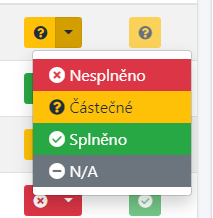
\includegraphics{img/ukazky/ctyrstavova_hodnota}
		\caption{Rozbalovací menu tlačítek pro čtyřstavovou hodnotu (zdroj: vlastní)}
		\label{fig:menu_tlacitek}
	\end{figure}
	\par Čtvrtá část obsahuje obecné informace o~projektu, týmu a mentorovi s~případnými prokliky. Karta také obsahuje odkazy na stránky třetích stran, které nastavuje vedoucí týmu. Nakonec se zde zobrazuje i informace o~udělených zápočtech a jednotlivé záznamy o~proběhlých obhajobách.
	\subsection{Mentorované projekty}
	\par Stránka mentorovaných projektů je důležitým rozcestníkem pro mentora. Uživatel zde má důležitou tabulku o~mentorovaných projektech a hlavně stručnou informaci o~postupu každého projektu (viz obrázek \ref{fig:postup_projektu}). Díky ukazateli postupu projektu mentor na první pohled vidí, jak si jednotlivé týmy vedou.
	\begin{figure}[H]
		\centering
		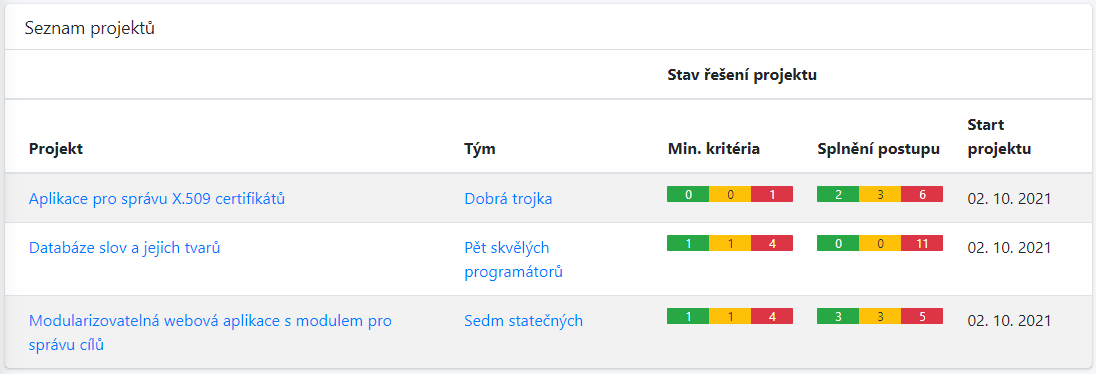
\includegraphics[width=\textwidth]{img/ukazky/mentorovane_projekty}
		\caption{Tabulka mentorovaných projektů (zdroj: vlastní)}
		\label{fig:postup_projektu}
	\end{figure}
\chapter{Testování}
	\par Jedním z~hlavních požadavků na výslednou aplikaci je její spolehlivost a robustnost. Tomu je podřízeno provedené rozsáhlé testování. Tvorba testů však není součástí této práce a je prováděna paralelní bakalářskou prací \uv{Komplexní testy webové aplikace} psanou Davidem Kůtou.
	\section{Testování aplikace}
	\par Aplikace byla připravována na různé druhy testů (viz \nameref{sec:testovatelnost}). Tyto testy byly vytvářeny současně při tvorbě aplikace, přičemž byl systém průběžně testován.
	\subsection{Jednotkové testování}
	\par Ačkoli jednotkové testování v~případě naší aplikace je velice omezené, je vytvořeno množství testů pro funkce pomocné třídy \texttt{Utils}. Tyto testy ověřují správnost výsledků funkcí na základě různých vstupních dat.
	\subsection{Automatické testování}
	\par Byly sestaveny automatické testy aplikace pomocí Selenium WebDriver Pro testování je automatickými testy kompletně dokončeno pokrytí rolí Vedoucí a Mentor. Pro roli Garant jsou dokončeny významné části přímo souvisejících s~organizací předmětů.
	\par Pro účely automatického testování byl připraven stav aplikace, kdy se v~datech systému vyskytuje většina možných stavů aplikace. Tento stav lze nahrát pomocí tlačítka \uv{ResetDB} umístěného v~liště horizontální navigace. Toto tlačítko přístupné pouze v~testovacím režimu aplikace.
	\subsection{End-to-end testy}
	\par Součástí testovací strategie jsou i testy, které otestují činnost aplikace v~sekvencí scénářů. Scénáře jsou vytvořeny dle předpokládaného způsobu užití aplikace.
	\subsection{Logování}
	\par Aplikace si také pro účely testování zaznamenává data o~provedených akcích. Při testování tedy možné sledovat posloupnost akcí, které se prováděly a které selhaly. Díky tomu lze jednoduše vysledovat příčinu nebo její přibližný výskyt.
	\subsection{Manuální testování}
	\par Některé funkce systému nebylo možné nebo přínosné testovat automaticky pomocí Selenium WebDriver. Typickým příkladem těchto částí aplikace je stahování a odesílání emailů. Proto tyto činnosti byly otestovány manuálně v~různých případech v~různých částech aplikace.
	\section{Výsledky testování}
	\par Po zahájení testování se objevila celá řada selhání. Většina nalezených defektů byla způsobena nedokončeným ošetřením přístupu na jednotlivé stránky nebo \hyphenation{ne-úpl-nos-tí} dat při práci s~databází. Veškeré defekty však byly původem implementačního rázu. Jednalo se tak o~odklad implementace od návrhu a dosud nebyl nalezen defekt, který by byl způsoben chybou návrhu aplikace.
	\par Nalezené odchylky od specifikace byly okamžitě po nalezení testerem komunikovány s~vývojářem a buď byla chyba na místě opravena nebo byl vytvořen záznam v~nástroji pro řízení projektu za účelem prošetření a případné opravy.  
\chapter{Závěr}
	\par V~bakalářské práci byla navržena a implementována webová aplikace, pro jejíž vývoj byl využity frameworky Nette a AdminLTE.
	Aplikace je středního rozsahu a svojí komplexností poměrně výrazně přesáhla původní odhady. Bylo vytvořeno 82 PHP souborů a dalších 185 pomocných souborů, o~celkové velikosti 249 MB zdrojového kódu (56,3 MB bez přiložených knihoven). Aplikace dává k~dispozici celkem 47 různých webových stránek.
	Při práci byly dodržovány všechny dobré postupy běžné v~současném SW vývoji, jako např. použití verzovacího systému, použití systému pro řízení projektu, použití systému pro správu incidentů. 
	Při vývoji byl kladen zvýšený důraz na robustnost, modularitu a testovatelnost aplikace. Vlastní testy ale byly prováděny v~rámci jiné bakalářské práce. Pozitivní význam důrazu na výše zmíněné vlastnosti se plně projevil již v~průběhu vývoje, neboť prototyp aplikace byl již v~prosinci 2021 podroben oponentuře budoucích uživatelů. A~na jejím základě vznikly četné požadavky na úpravy, změny a doplnění. Díky výše zmíněným vlastnostem aplikace bylo možné tyto požadavky beze zbytku provést a otestovat.
	Vyvinutá aplikace svojí realizovanou funkcionalitou splňuje všechny požadavky na nasazení v~předmětu KIV/TSP1.
	
	V~současné době je aplikace nasazena na vývojovém prostředí. Úplné dokončení aplikace, tj. její nasazení na katedrální server a doladění všech přístupových práv, je plánováno v~období srpen až září 2022 tak, aby již v~ZS akademického roku 2022/23 mohli aplikaci využívat vyučující i studenti předmětu KIV/TSP1.
	\section{Další možný vývoj}
	\par Aplikace má mnoho potenciálu jak v~univerzitním prostředí růst. Jedním z~další možných rozšíření je implementace přihlášení skrz protokol Kerberos univerzitní sítě a umožnit tak jednotné přihlášení do aplikace. To by mohlo znamenat i možnost nové role Student, jejíž držitelé by si mohli prohlížet aktuální stav svého týmu a projektu a případně kontrolovat akce svého vedoucího.
	\par Dalším rozšířením aplikace je přidat podporu pro netypické případy studia předmětů TSP (např. studium pouze jednoho z~předmětů).
	\par V~neposlední řadě také byl předložen nápad do budoucna rozšířit software i do dalších předmětů podobného zaměření (KIV/ASWI, KIV/ZSWI, atd.).
\listoffigures
%
% SEZNAM UKÁZEK KÓDU
%
\lstlistoflistings
% 

\chapter*{Seznam použitých zkratek}
% \printglossaries
\begin{description}
	\item[PHP] Hypertextový preprocesor
	\item[HTML] Hyper Text Markup Language
	\item[SGML] Standard Generalized Markup Language
	\item[CSS] Cascading Style Sheet
	\item[PDF] Portable Document Format
	\item[CSV] Comma-separated values
	\item[UC] Use Case
	\item[DI] Dependency Injection
	\item[MVC] Třívrstvá architektura Model-View-Controller
	\item[MVP] Třívrstvá architektura Model-View-Presenter
	\item[SQL] Structured Query Language
	\item[YAML] YAML Ain't Markup Language
	\item[KIV] Katedra informatiky a výpočetní techniky
	\item[TSP] Týmový softwarový projekt
	\item[PSTSP] Podpůrný software TSP
\end{description}
% PRO ANGLICKOU SAZBU JE NUTNÉ ZMĚNIT
% CITAČNÍ STYL!
%
\bibliographystyle{csplainnatkiv}
{\raggedright\small
\bibliography{literatura}

\appendix
\chapter{Případy užití}
Případy užití jsou sestaveny v~originální XML struktuře následně vygenerované do čitelné HTML podoby. Následující obrázek \ref{fig:uc_example} představuje ukázku těchto vygenerovaných výstupů. Veškeré sepsané případy užití jsou součástí obsahu odevzdané práce. Případy jsou očíslovány dle tabulky \ref{tab:use-case-table}.

\begin{figure}[H]
	\centering
	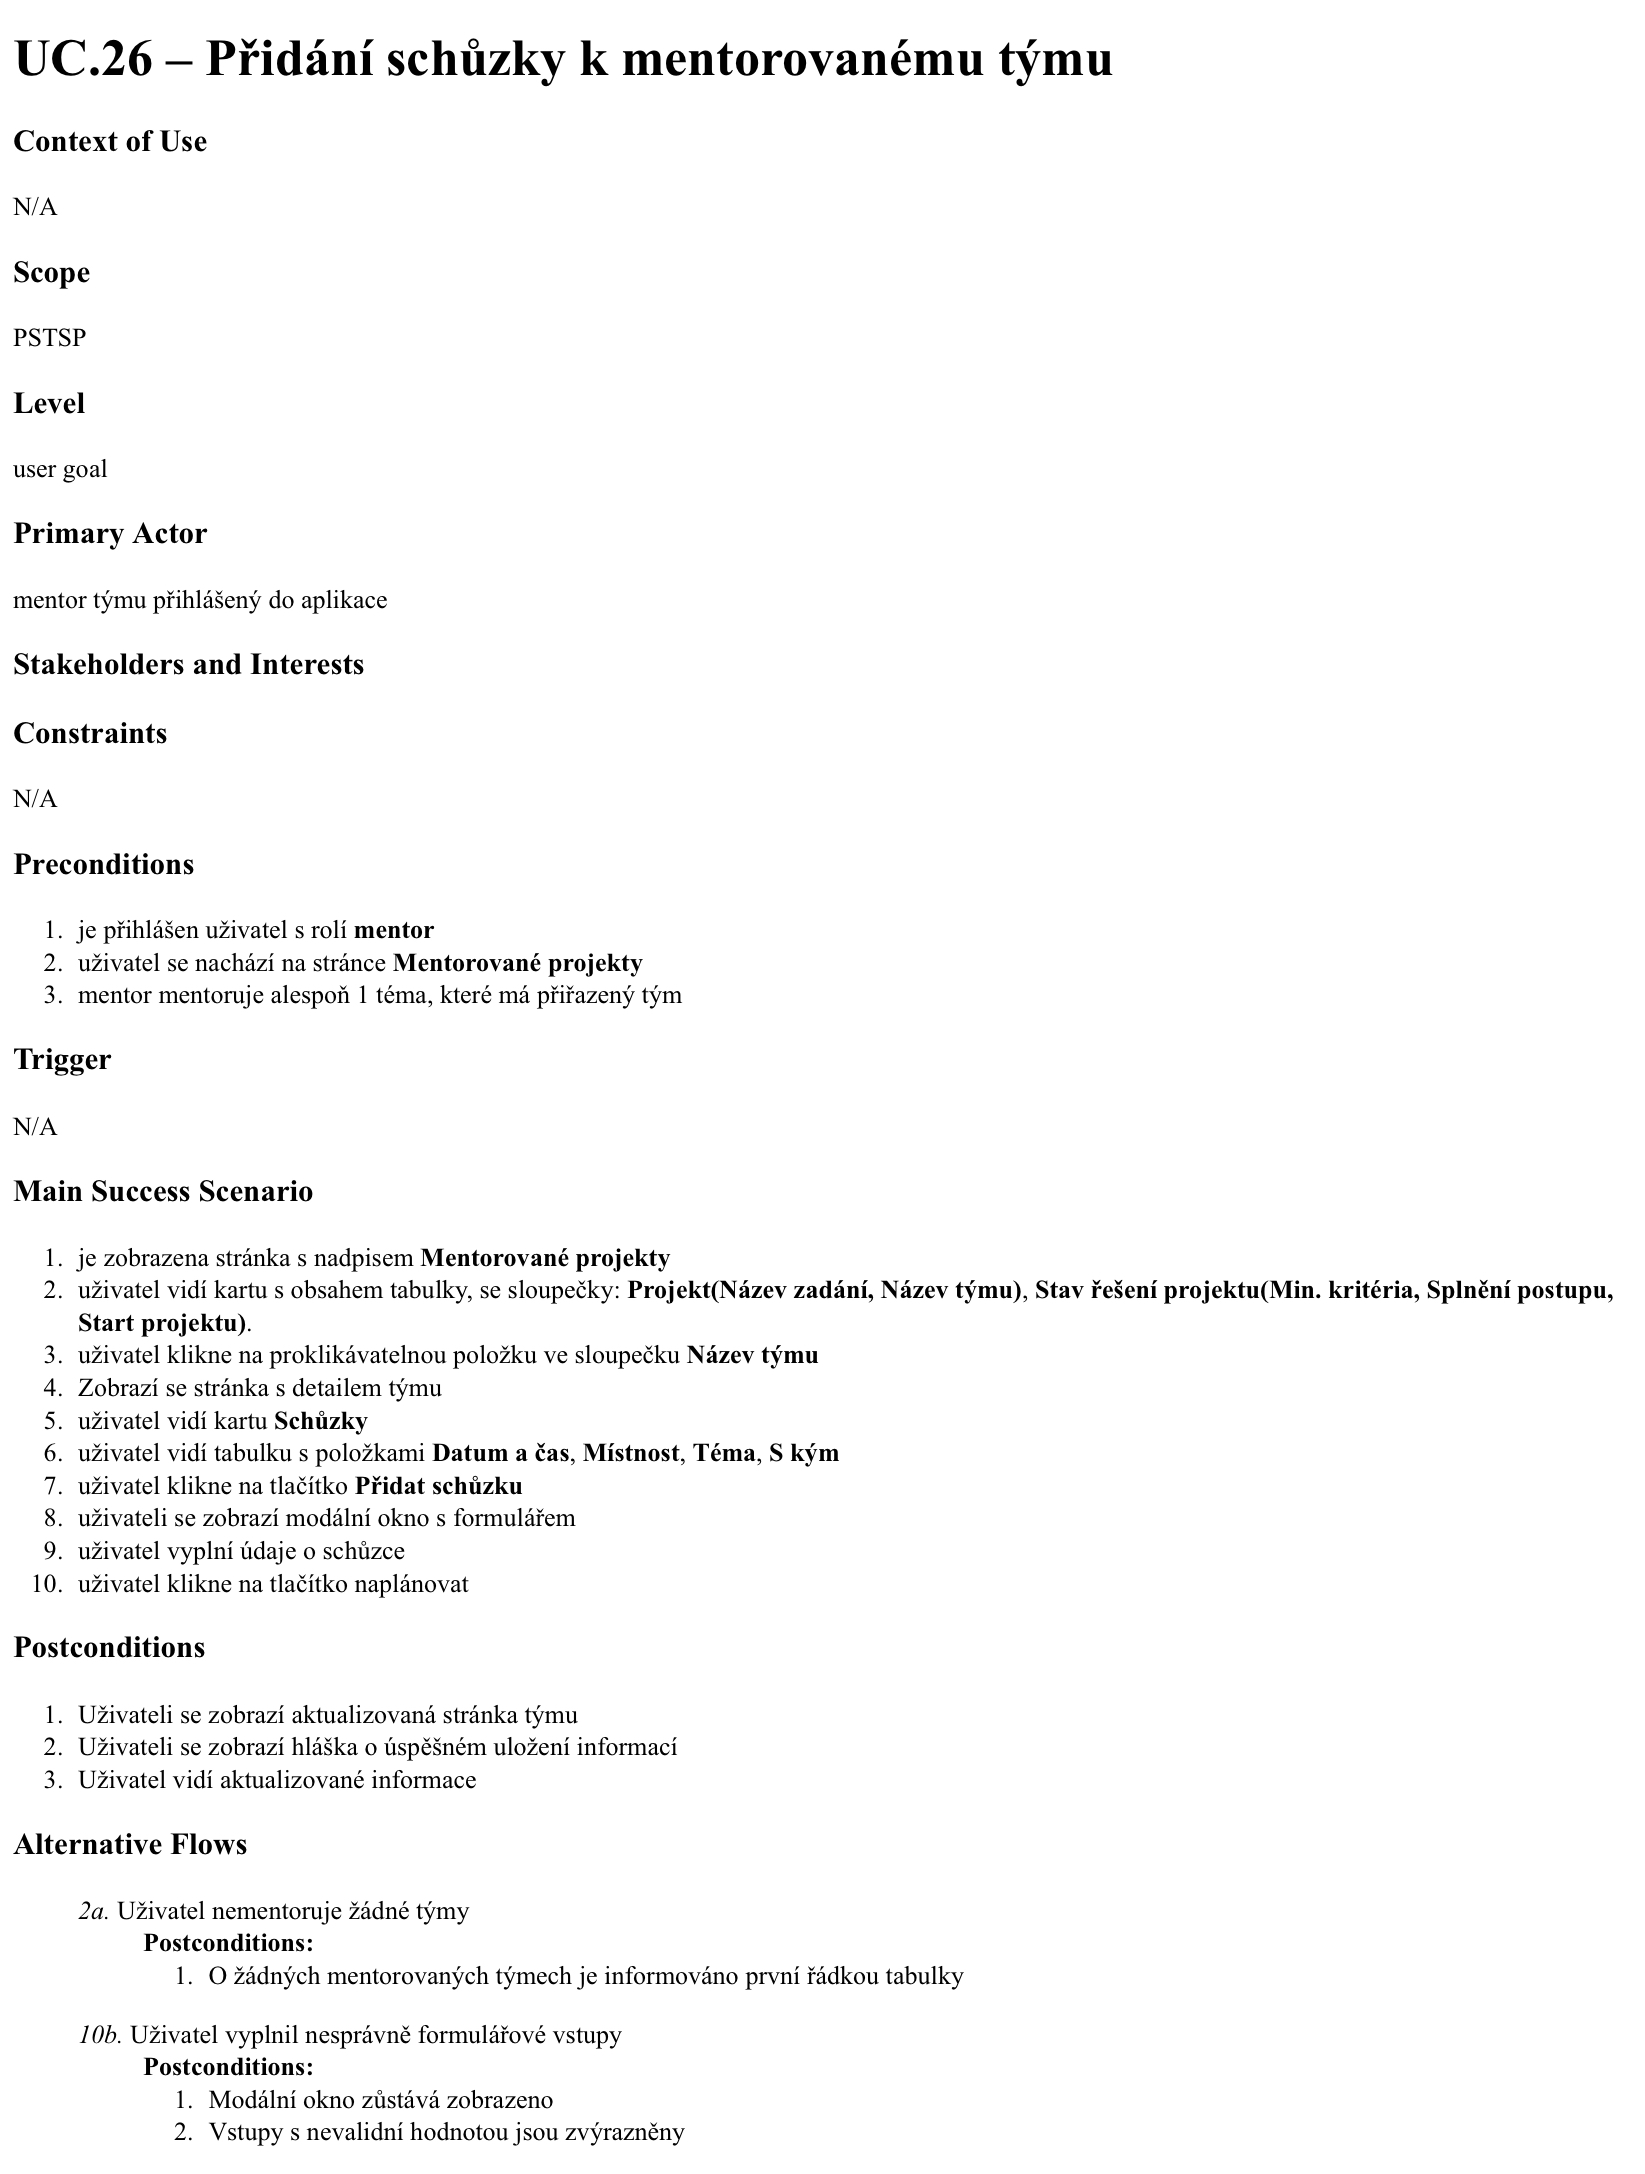
\includegraphics[width=0.9\textwidth]{img/use_case/use_case_example}
	\caption{Ukázka sepsaného UC (zdroj: vlastní)}
	\label{fig:uc_example}
\end{figure}

\begin{table}[]
	\caption{Seznam případů užití}
	\label{tab:use-case-table}
	\centering
	\begin{xltabular}{\textwidth}{|r|X|}\hline
		Číslo UC & Popis\\\hline\hline
		UC.01	& Přihlášení do aplikace\\\hline
		UC.02	& Zobrazení seznamu témat\\\hline
		UC.02	& Zobrazení detailu tématu\\\hline
		UC.03	& Zobrazení neúplných týmů\\\hline
		UC.04	& Odhlášení přihlášeného uživatele\\\hline
		UC.05	& Zobrazení schůzek týmu\\\hline
		UC.06	& Přidání schůzky týmu\\\hline
		UC.07	& Zobrazení podrobného zápisu ze schůzky\\\hline
		UC.08	& Zobrazení podrobného zápisu ze schůzky\\\hline
		UC.09	& Přidání podrobného zápisu ze schůzky\\\hline
		UC.10	& Zobrazení stavu řešení projektu\\\hline
		UC.11	& Změna stavu řešení projektu\\\hline
		UC.12	& Změna stavu řešení projektu - přidání využité zkušennosti\\\hline
		UC.13	& Úprava odkazů k~projektu\\\hline
		UC.14	& Manipulace se členy týmu\\\hline
		UC.15	& Nastavení informací o~členech týmu\\\hline
		UC.16	& Nastavení profilu týmu\\\hline
		UC.17	& Projevení zájmu o~téma pro svůj tým\\\hline
		UC.18	& Zobrazení témat, o~které tým projevil zájem\\\hline
		UC.19	& Zobrazení přiděleného tématu\\\hline
		UC.20	& Změna kontaktních informací u~mentora\\\hline
		UC.21	& Zobrazení mentorovaných projektů\\\hline
		UC.22	& Zobrazení stavu řešení projektu u~mentorovaného týmu\\\hline
		UC.23	& Změna stavu řešení projektu u~mentorovaného týmu\\\hline
		UC.24	& Zobrazení týmu řešící mentorovaný projekt\\\hline
		UC.25	& Zobrazení tématu u~mentorovaného týmu\\\hline
		UC.26	& Přidání schůzky k~mentorovanému týmu\\\hline
		UC.27	& Zobrazení nementorovaných témat\\\hline
		UC.28	& Přiřazení tématu mentorovi\\\hline
		UC.29	& Zobrazení témat bez týmu\\\hline
		UC.30	& Stanovení vhodnosti tématu k~týmu, který o~toto téma projevil zájem\\\hline 
	\end{xltabular}

\end{table}
\begin{table}
	\begin{xltabular}{\textwidth}{|r|X|}\hline
		Číslo UC & Popis\\\hline\hline
		UC.31	& Zobrazení historie mentorovaných témat\\\hline
		UC.32	& Zobrazení témat bez mentora\\\hline
		UC.33	& Zobrazení seznamu týmů\\\hline
		UC.34	& Editace týmů ze seznamu týmů\\\hline
		UC.35	& Editace zápočtů týmu ze seznamu týmů\\\hline
		UC.36	& Přidání záznamu o~obhajobě\\\hline
		UC.37	& Zobrazení tabulky projektů mentorů\\\hline
		UC.38	& Zobrazení pohledu mentora\\\hline
		UC.39	& Správa uživatelů - zobrazení\\\hline
		UC.40	& Odebrání uživatele\\\hline
		UC.41	& Přidání mentora\\\hline
		UC.42	& Správa zadání\\\hline
		UC.43	& Přidání nového tématu\\\hline
		UC.44	& Zobrazení správy štítků\\\hline
		UC.45	& Přidání týmové role\\\hline
		UC.46	& Úprava týmové role\\\hline
		UC.47	& Přidání profilu týmu\\\hline
		UC.48	& Úprava profilu týmu\\\hline
		UC.49	& Zobrazení tabulky přidělení\\\hline
		UC.50	& Přiřazení tématu týmu\\\hline
		UC.51	& Zobrazení správy studentů\\\hline
		UC.52	& Přidání studenta\\\hline
		UC.53	& Import studentů z~CSV souboru\\\hline
		UC.54	& Smazání studenta\\\hline
		UC.55	& Vytvoření týmu\\\hline
		UC.56	& Vytvoření nového ročníku\\\hline
		UC.57	& Nastavení aktuální ročníku\\\hline
		UC.58	& Zobrazení záznamu logu\\\hline
		UC.59	& Stažení záznamu logu\\\hline
		
	\end{xltabular}
\end{table}
\chapter{Databázový EER model}

\begin{figure}[H]
	\centering
	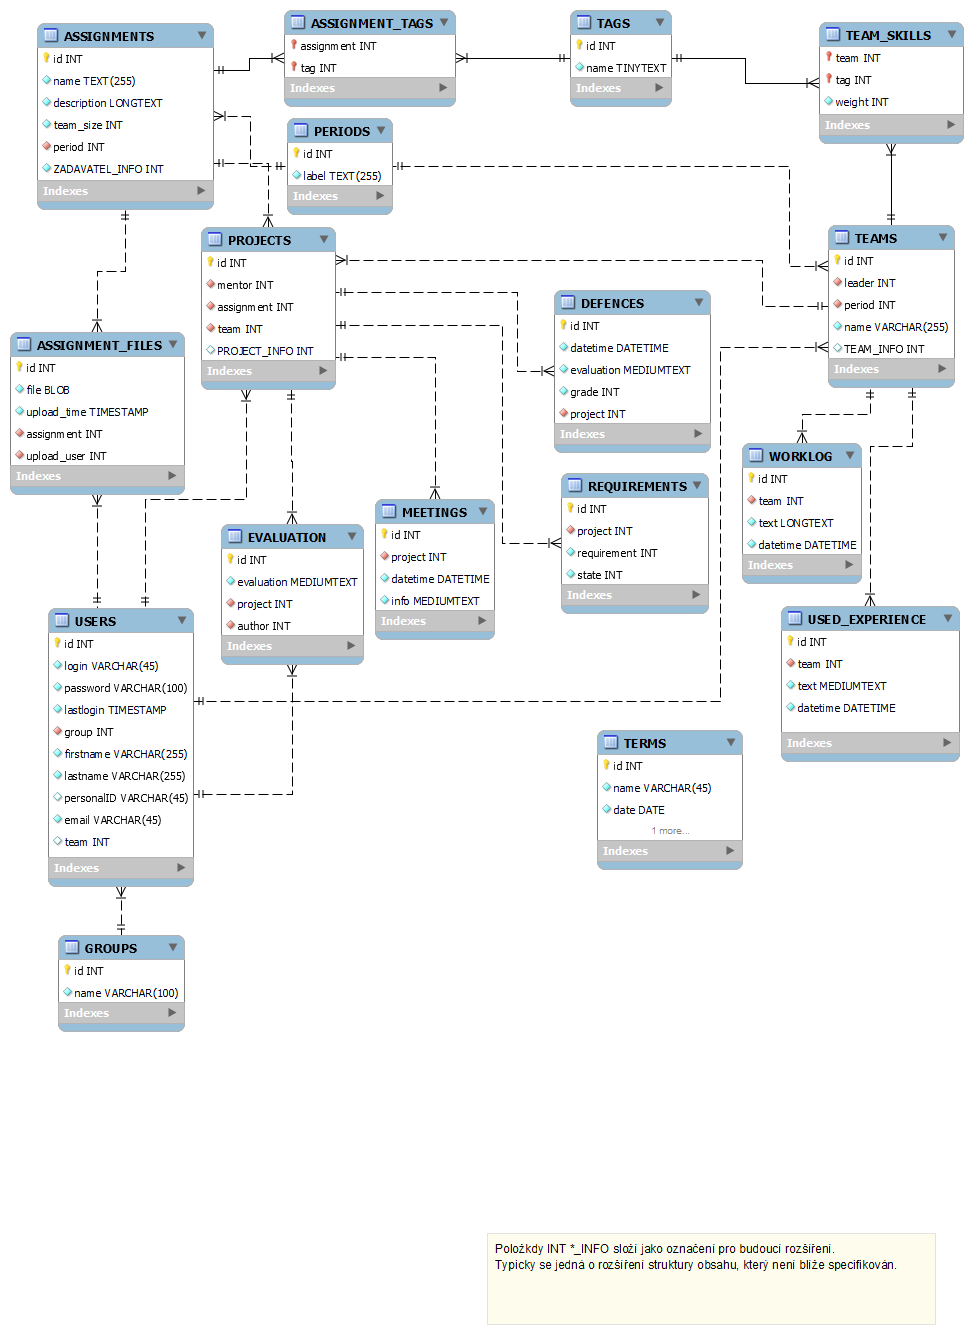
\includegraphics[width=1\textwidth]{img/database/database_model}
	\caption{EER model diagram (zdroj: vlastní)}
	\label{fig:uc_example}
\end{figure}
\chapter{Obsah elektronické přílohy}
\section{Adresářová struktura}

\dirtree{%
.1 /.
	.2 Aplikace\_a\_knihovny.
		.3 Aplikace \normalfont{-- projekt webové aplikace}.
		.3 EER\_DB\_model \normalfont{-- EER model databáze}.
			.4 database\_model.mwb \normalfont{-- model databáze ve formátu MWB (MySQL Workbench)}.
			.4 eer\_model\_diagram.svg \normalfont{-- EER model diagram databázové struktury ve formátu SVG}.
		.3 SQL\_skripty \normalfont{-- SQL skripty pro vytvoření databáze}.
			.4 PSTSP\_DB\_structure.sql \normalfont{-- SQL skript pro vytvoření struktury databáze}.
			.4 PSTSP\_DB\_structure\_data1.sql \normalfont{-- SQL skript pro vytvoření struktury databáze a naplnění 1. variantou testovacích dat}.
			.4 PSTSP\_DB\_structure\_data2.sql \normalfont{-- SQL skript pro vytvoření struktury databáze a naplnění 2. variantou testovacích dat}.
		.3 UC.
			.4 diagram.
				.5 use-case-diagram.png \normalfont{-- diagram případů užití ve formátu PNG}.
				.5 use-case-diagram.uxf \normalfont{-- diagram případů užití ve formátu UXF (UMLet)}.
			.4 html \normalfont{-- případy užití ve formátu HTML}.
			.4 xml \normalfont{-- případy užití ve formátu XML}.
	.2 Text\_prace \normalfont{-- konfigurační soubory}.
		.3 tex \normalfont{-- zdrojové soubory \TeX včetně přiložených souborů}.
		.3 A19B0052P \normalfont{-- bakalářská práce ve formátu PDF}.
	.2 readme.txt \normalfont{-- popis adresářové struktury}.
}


\end{document}
